\documentclass{article}

%Para hacer encabezados
\usepackage{fancyhdr,lipsum}

%Formato de las tablas
\usepackage[table,xcdraw]{xcolor}

%Hacer comentarios
\usepackage{verbatim}

%Cancelar cosas de mate
\usepackage{cancel}

%Para uso de links
% \usepackage{hyperref}

% para las imagenes
\usepackage{float}

%Para escribir codigo bonito
\usepackage[newfloat]{minted}
\usepackage{caption}
\usepackage{lmodern}
\usepackage{minted}

\newenvironment{code}{\captionsetup{type=listing}}{}

%usar matrices
\usepackage{amsmath}

%Para usar símbolos matemáticos
\usepackage{amssymb}
\usepackage{amsmath}

%Para poder utilizar las tildes en español
%\usepackage[spanish]{babel}
%\usepackage[utf8]{inputenc}

%Para poder escribir distintos lenguajes
\usepackage{listings}

%Para poder decodificar letras con acento
\usepackage[T1]{fontenc}

%Definición del comando que equivale a una tabulación
\newcommand\tab[1][1cm]{\hspace*{#1}}

%Para poder insertar imagenes y definir el path donde estan
\usepackage{graphicx}
\graphicspath{ {img/} }

%Esto es para eliminar el corte de palabras
\usepackage[none]{hyphenat}

%Esto es para poder definir colores
\usepackage{color}

%Esto es para poder cambiar los margenes
\usepackage{vmargin}

%Para usar tablas especiales
\usepackage{tabularx}

%PARA MANEJAR CODIGO PYTHON EN LATEX------------------------------------------------

\usepackage[breakable]{tcolorbox}
\usepackage{parskip} % Stop auto-indenting (to mimic markdown behaviour)
\setkeys{Gin}{keepaspectratio}
\let\Oldincludegraphics\includegraphics
\usepackage{caption}
% \DeclareCaptionFormat{nocaption}{}
% \captionsetup{format=nocaption,aboveskip=0pt,belowskip=0pt}

\usepackage{float}
\floatplacement{figure}{H} % forces figures to be placed at the correct location
\usepackage{xcolor} % Allow colors to be defined
\usepackage{enumerate} % Needed for markdown enumerations to work
\usepackage{geometry} % Used to adjust the document margins
\usepackage{amsmath} % Equations
\usepackage{amssymb} % Equations
\usepackage{textcomp} % defines textquotesingle
% Hack from http://tex.stackexchange.com/a/47451/13684:
\AtBeginDocument{%
    \def\PYZsq{\textquotesingle}% Upright quotes in Pygmentized code
}

\usepackage{upquote} % Upright quotes for verbatim code
\usepackage{eurosym} % defines \euro

\usepackage{iftex}
    \ifPDFTeX
        \usepackage[T1]{fontenc}
        \IfFileExists{alphabeta.sty}{
              \usepackage{alphabeta}
          }{
              \usepackage[mathletters]{ucs}
              \usepackage[utf8x]{inputenc}
          }
    \else
        \usepackage{fontspec}
        \usepackage{unicode-math}
    \fi

    \usepackage{fancyvrb} % verbatim replacement that allows latex
    \usepackage{grffile} % extends the file name processing of package graphics
                         % to support a larger range
    \makeatletter % fix for old versions of grffile with XeLaTeX
    \@ifpackagelater{grffile}{2019/11/01}
    {
      % Do nothing on new versions
    }
    {
      \def\Gread@@xetex#1{%
        \IfFileExists{"\Gin@base".bb}%
        {\Gread@eps{\Gin@base.bb}}%
        {\Gread@@xetex@aux#1}%
      }
    }

\makeatother
\usepackage[Export]{adjustbox} % Used to constrain images to a maximum size
\adjustboxset{max size={0.9\linewidth}{0.9\paperheight}}

% The hyperref package gives us a pdf with properly built
% internal navigation ('pdf bookmarks' for the table of contents,
% internal cross-reference links, web links for URLs, etc.)
\usepackage{hyperref}
% The default LaTeX title has an obnoxious amount of whitespace. By default,
% titling removes some of it. It also provides customization options.
\usepackage{titling}
\usepackage{longtable} % longtable support required by pandoc >1.10
\usepackage{booktabs}  % table support for pandoc > 1.12.2
\usepackage{array}     % table support for pandoc >= 2.11.3
\usepackage{calc}      % table minipage width calculation for pandoc >= 2.11.1
\usepackage[inline]{enumitem} % IRkernel/repr support (it uses the enumerate* environment)
\usepackage[normalem]{ulem} % ulem is needed to support strikethroughs (\sout)
                                % normalem makes italics be italics, not underlines
\usepackage{soul}      % strikethrough (\st) support for pandoc >= 3.0.0
\usepackage{mathrsfs}

    % Colors for the hyperref package
    \definecolor{urlcolor}{rgb}{0,.145,.698}
    \definecolor{linkcolor}{rgb}{.71,0.21,0.01}
    \definecolor{citecolor}{rgb}{.12,.54,.11}

    % ANSI colors
    \definecolor{ansi-black}{HTML}{3E424D}
    \definecolor{ansi-black-intense}{HTML}{282C36}
    \definecolor{ansi-red}{HTML}{E75C58}
    \definecolor{ansi-red-intense}{HTML}{B22B31}
    \definecolor{ansi-green}{HTML}{00A250}
    \definecolor{ansi-green-intense}{HTML}{007427}
    \definecolor{ansi-yellow}{HTML}{DDB62B}
    \definecolor{ansi-yellow-intense}{HTML}{B27D12}
    \definecolor{ansi-blue}{HTML}{208FFB}
    \definecolor{ansi-blue-intense}{HTML}{0065CA}
    \definecolor{ansi-magenta}{HTML}{D160C4}
    \definecolor{ansi-magenta-intense}{HTML}{A03196}
    \definecolor{ansi-cyan}{HTML}{60C6C8}
    \definecolor{ansi-cyan-intense}{HTML}{258F8F}
    \definecolor{ansi-white}{HTML}{C5C1B4}
    \definecolor{ansi-white-intense}{HTML}{A1A6B2}
    \definecolor{ansi-default-inverse-fg}{HTML}{FFFFFF}
    \definecolor{ansi-default-inverse-bg}{HTML}{000000}

    \definecolor{outerrorbackground}{HTML}{FFDFDF}

    % commands and environments needed by pandoc snippets
    % extracted from the output of `pandoc -s`
    \providecommand{\tightlist}{%
      \setlength{\itemsep}{0pt}\setlength{\parskip}{0pt}}
    \DefineVerbatimEnvironment{Highlighting}{Verbatim}{commandchars=\\\{\}}
    % Add ',fontsize=\small' for more characters per line
    \newenvironment{Shaded}{}{}
    \newcommand{\KeywordTok}[1]{\textcolor[rgb]{0.00,0.44,0.13}{\textbf{{#1}}}}
    \newcommand{\DataTypeTok}[1]{\textcolor[rgb]{0.56,0.13,0.00}{{#1}}}
    \newcommand{\DecValTok}[1]{\textcolor[rgb]{0.25,0.63,0.44}{{#1}}}
    \newcommand{\BaseNTok}[1]{\textcolor[rgb]{0.25,0.63,0.44}{{#1}}}
    \newcommand{\FloatTok}[1]{\textcolor[rgb]{0.25,0.63,0.44}{{#1}}}
    \newcommand{\CharTok}[1]{\textcolor[rgb]{0.25,0.44,0.63}{{#1}}}
    \newcommand{\StringTok}[1]{\textcolor[rgb]{0.25,0.44,0.63}{{#1}}}
    \newcommand{\CommentTok}[1]{\textcolor[rgb]{0.38,0.63,0.69}{\textit{{#1}}}}
    \newcommand{\OtherTok}[1]{\textcolor[rgb]{0.00,0.44,0.13}{{#1}}}
    \newcommand{\AlertTok}[1]{\textcolor[rgb]{1.00,0.00,0.00}{\textbf{{#1}}}}
    \newcommand{\FunctionTok}[1]{\textcolor[rgb]{0.02,0.16,0.49}{{#1}}}
    \newcommand{\RegionMarkerTok}[1]{{#1}}
    \newcommand{\ErrorTok}[1]{\textcolor[rgb]{1.00,0.00,0.00}{\textbf{{#1}}}}
    \newcommand{\NormalTok}[1]{{#1}}

        % Additional commands for more recent versions of Pandoc
    \newcommand{\ConstantTok}[1]{\textcolor[rgb]{0.53,0.00,0.00}{{#1}}}
    \newcommand{\SpecialCharTok}[1]{\textcolor[rgb]{0.25,0.44,0.63}{{#1}}}
    \newcommand{\VerbatimStringTok}[1]{\textcolor[rgb]{0.25,0.44,0.63}{{#1}}}
    \newcommand{\SpecialStringTok}[1]{\textcolor[rgb]{0.73,0.40,0.53}{{#1}}}
    \newcommand{\ImportTok}[1]{{#1}}
    \newcommand{\DocumentationTok}[1]{\textcolor[rgb]{0.73,0.13,0.13}{\textit{{#1}}}}
    \newcommand{\AnnotationTok}[1]{\textcolor[rgb]{0.38,0.63,0.69}{\textbf{\textit{{#1}}}}}
    \newcommand{\CommentVarTok}[1]{\textcolor[rgb]{0.38,0.63,0.69}{\textbf{\textit{{#1}}}}}
    \newcommand{\VariableTok}[1]{\textcolor[rgb]{0.10,0.09,0.49}{{#1}}}
    \newcommand{\ControlFlowTok}[1]{\textcolor[rgb]{0.00,0.44,0.13}{\textbf{{#1}}}}
    \newcommand{\OperatorTok}[1]{\textcolor[rgb]{0.40,0.40,0.40}{{#1}}}
    \newcommand{\BuiltInTok}[1]{{#1}}
    \newcommand{\ExtensionTok}[1]{{#1}}
    \newcommand{\PreprocessorTok}[1]{\textcolor[rgb]{0.74,0.48,0.00}{{#1}}}
    \newcommand{\AttributeTok}[1]{\textcolor[rgb]{0.49,0.56,0.16}{{#1}}}
    \newcommand{\InformationTok}[1]{\textcolor[rgb]{0.38,0.63,0.69}{\textbf{\textit{{#1}}}}}
    \newcommand{\WarningTok}[1]{\textcolor[rgb]{0.38,0.63,0.69}{\textbf{\textit{{#1}}}}}
    \makeatletter
    \newsavebox\pandoc@box
        \newcommand*\pandocbounded[1]{%
      \sbox\pandoc@box{#1}%
      % scaling factors for width and height
      \Gscale@div\@tempa\textheight{\dimexpr\ht\pandoc@box+\dp\pandoc@box\relax}%
      \Gscale@div\@tempb\linewidth{\wd\pandoc@box}%
      % select the smaller of both
      \ifdim\@tempb\p@<\@tempa\p@
        \let\@tempa\@tempb
      \fi
      % scaling accordingly (\@tempa < 1)
      \ifdim\@tempa\p@<\p@
        \scalebox{\@tempa}{\usebox\pandoc@box}%
      % scaling not needed, use as it is
      \else
        \usebox{\pandoc@box}%
      \fi
    }
    \makeatother

    % Define a nice break command that doesn't care if a line doesn't already
    % exist.
    \def\br{\hspace*{\fill} \\* }
    % Math Jax compatibility definitions
    \def\gt{>}
    \def\lt{<}
    \let\Oldtex\TeX
    \let\Oldlatex\LaTeX
    \renewcommand{\TeX}{\textrm{\Oldtex}}
    \renewcommand{\LaTeX}{\textrm{\Oldlatex}}

    \makeatletter
\def\PY@reset{\let\PY@it=\relax \let\PY@bf=\relax%
    \let\PY@ul=\relax \let\PY@tc=\relax%
    \let\PY@bc=\relax \let\PY@ff=\relax}
\def\PY@tok#1{\csname PY@tok@#1\endcsname}
\def\PY@toks#1+{\ifx\relax#1\empty\else%
    \PY@tok{#1}\expandafter\PY@toks\fi}
\def\PY@do#1{\PY@bc{\PY@tc{\PY@ul{%
    \PY@it{\PY@bf{\PY@ff{#1}}}}}}}
\def\PY#1#2{\PY@reset\PY@toks#1+\relax+\PY@do{#2}}

\@namedef{PY@tok@w}{\def\PY@tc##1{\textcolor[rgb]{0.73,0.73,0.73}{##1}}}
\@namedef{PY@tok@c}{\let\PY@it=\textit\def\PY@tc##1{\textcolor[rgb]{0.24,0.48,0.48}{##1}}}
\@namedef{PY@tok@cp}{\def\PY@tc##1{\textcolor[rgb]{0.61,0.40,0.00}{##1}}}
\@namedef{PY@tok@k}{\let\PY@bf=\textbf\def\PY@tc##1{\textcolor[rgb]{0.00,0.50,0.00}{##1}}}
\@namedef{PY@tok@kp}{\def\PY@tc##1{\textcolor[rgb]{0.00,0.50,0.00}{##1}}}
\@namedef{PY@tok@kt}{\def\PY@tc##1{\textcolor[rgb]{0.69,0.00,0.25}{##1}}}
\@namedef{PY@tok@o}{\def\PY@tc##1{\textcolor[rgb]{0.40,0.40,0.40}{##1}}}
\@namedef{PY@tok@ow}{\let\PY@bf=\textbf\def\PY@tc##1{\textcolor[rgb]{0.67,0.13,1.00}{##1}}}
\@namedef{PY@tok@nb}{\def\PY@tc##1{\textcolor[rgb]{0.00,0.50,0.00}{##1}}}
\@namedef{PY@tok@nf}{\def\PY@tc##1{\textcolor[rgb]{0.00,0.00,1.00}{##1}}}
\@namedef{PY@tok@nc}{\let\PY@bf=\textbf\def\PY@tc##1{\textcolor[rgb]{0.00,0.00,1.00}{##1}}}
\@namedef{PY@tok@nn}{\let\PY@bf=\textbf\def\PY@tc##1{\textcolor[rgb]{0.00,0.00,1.00}{##1}}}
\@namedef{PY@tok@ne}{\let\PY@bf=\textbf\def\PY@tc##1{\textcolor[rgb]{0.80,0.25,0.22}{##1}}}
\@namedef{PY@tok@nv}{\def\PY@tc##1{\textcolor[rgb]{0.10,0.09,0.49}{##1}}}
\@namedef{PY@tok@no}{\def\PY@tc##1{\textcolor[rgb]{0.53,0.00,0.00}{##1}}}
\@namedef{PY@tok@nl}{\def\PY@tc##1{\textcolor[rgb]{0.46,0.46,0.00}{##1}}}
\@namedef{PY@tok@ni}{\let\PY@bf=\textbf\def\PY@tc##1{\textcolor[rgb]{0.44,0.44,0.44}{##1}}}
\@namedef{PY@tok@na}{\def\PY@tc##1{\textcolor[rgb]{0.41,0.47,0.13}{##1}}}
\@namedef{PY@tok@nt}{\let\PY@bf=\textbf\def\PY@tc##1{\textcolor[rgb]{0.00,0.50,0.00}{##1}}}
\@namedef{PY@tok@nd}{\def\PY@tc##1{\textcolor[rgb]{0.67,0.13,1.00}{##1}}}
\@namedef{PY@tok@s}{\def\PY@tc##1{\textcolor[rgb]{0.73,0.13,0.13}{##1}}}
\@namedef{PY@tok@sd}{\let\PY@it=\textit\def\PY@tc##1{\textcolor[rgb]{0.73,0.13,0.13}{##1}}}
\@namedef{PY@tok@si}{\let\PY@bf=\textbf\def\PY@tc##1{\textcolor[rgb]{0.64,0.35,0.47}{##1}}}
\@namedef{PY@tok@se}{\let\PY@bf=\textbf\def\PY@tc##1{\textcolor[rgb]{0.67,0.36,0.12}{##1}}}
\@namedef{PY@tok@sr}{\def\PY@tc##1{\textcolor[rgb]{0.64,0.35,0.47}{##1}}}
\@namedef{PY@tok@ss}{\def\PY@tc##1{\textcolor[rgb]{0.10,0.09,0.49}{##1}}}
\@namedef{PY@tok@sx}{\def\PY@tc##1{\textcolor[rgb]{0.00,0.50,0.00}{##1}}}
\@namedef{PY@tok@m}{\def\PY@tc##1{\textcolor[rgb]{0.40,0.40,0.40}{##1}}}
\@namedef{PY@tok@gh}{\let\PY@bf=\textbf\def\PY@tc##1{\textcolor[rgb]{0.00,0.00,0.50}{##1}}}
\@namedef{PY@tok@gu}{\let\PY@bf=\textbf\def\PY@tc##1{\textcolor[rgb]{0.50,0.00,0.50}{##1}}}
\@namedef{PY@tok@gd}{\def\PY@tc##1{\textcolor[rgb]{0.63,0.00,0.00}{##1}}}
\@namedef{PY@tok@gi}{\def\PY@tc##1{\textcolor[rgb]{0.00,0.52,0.00}{##1}}}
\@namedef{PY@tok@gr}{\def\PY@tc##1{\textcolor[rgb]{0.89,0.00,0.00}{##1}}}
\@namedef{PY@tok@ge}{\let\PY@it=\textit}
\@namedef{PY@tok@gs}{\let\PY@bf=\textbf}
\@namedef{PY@tok@ges}{\let\PY@bf=\textbf\let\PY@it=\textit}
\@namedef{PY@tok@gp}{\let\PY@bf=\textbf\def\PY@tc##1{\textcolor[rgb]{0.00,0.00,0.50}{##1}}}
\@namedef{PY@tok@go}{\def\PY@tc##1{\textcolor[rgb]{0.44,0.44,0.44}{##1}}}
\@namedef{PY@tok@gt}{\def\PY@tc##1{\textcolor[rgb]{0.00,0.27,0.87}{##1}}}
\@namedef{PY@tok@err}{\def\PY@bc##1{{\setlength{\fboxsep}{\string -\fboxrule}\fcolorbox[rgb]{1.00,0.00,0.00}{1,1,1}{\strut ##1}}}}
\@namedef{PY@tok@kc}{\let\PY@bf=\textbf\def\PY@tc##1{\textcolor[rgb]{0.00,0.50,0.00}{##1}}}
\@namedef{PY@tok@kd}{\let\PY@bf=\textbf\def\PY@tc##1{\textcolor[rgb]{0.00,0.50,0.00}{##1}}}
\@namedef{PY@tok@kn}{\let\PY@bf=\textbf\def\PY@tc##1{\textcolor[rgb]{0.00,0.50,0.00}{##1}}}
\@namedef{PY@tok@kr}{\let\PY@bf=\textbf\def\PY@tc##1{\textcolor[rgb]{0.00,0.50,0.00}{##1}}}
\@namedef{PY@tok@bp}{\def\PY@tc##1{\textcolor[rgb]{0.00,0.50,0.00}{##1}}}
\@namedef{PY@tok@fm}{\def\PY@tc##1{\textcolor[rgb]{0.00,0.00,1.00}{##1}}}
\@namedef{PY@tok@vc}{\def\PY@tc##1{\textcolor[rgb]{0.10,0.09,0.49}{##1}}}
\@namedef{PY@tok@vg}{\def\PY@tc##1{\textcolor[rgb]{0.10,0.09,0.49}{##1}}}
\@namedef{PY@tok@vi}{\def\PY@tc##1{\textcolor[rgb]{0.10,0.09,0.49}{##1}}}
\@namedef{PY@tok@vm}{\def\PY@tc##1{\textcolor[rgb]{0.10,0.09,0.49}{##1}}}
\@namedef{PY@tok@sa}{\def\PY@tc##1{\textcolor[rgb]{0.73,0.13,0.13}{##1}}}
\@namedef{PY@tok@sb}{\def\PY@tc##1{\textcolor[rgb]{0.73,0.13,0.13}{##1}}}
\@namedef{PY@tok@sc}{\def\PY@tc##1{\textcolor[rgb]{0.73,0.13,0.13}{##1}}}
\@namedef{PY@tok@dl}{\def\PY@tc##1{\textcolor[rgb]{0.73,0.13,0.13}{##1}}}
\@namedef{PY@tok@s2}{\def\PY@tc##1{\textcolor[rgb]{0.73,0.13,0.13}{##1}}}
\@namedef{PY@tok@sh}{\def\PY@tc##1{\textcolor[rgb]{0.73,0.13,0.13}{##1}}}
\@namedef{PY@tok@s1}{\def\PY@tc##1{\textcolor[rgb]{0.73,0.13,0.13}{##1}}}
\@namedef{PY@tok@mb}{\def\PY@tc##1{\textcolor[rgb]{0.40,0.40,0.40}{##1}}}
\@namedef{PY@tok@mf}{\def\PY@tc##1{\textcolor[rgb]{0.40,0.40,0.40}{##1}}}
\@namedef{PY@tok@mh}{\def\PY@tc##1{\textcolor[rgb]{0.40,0.40,0.40}{##1}}}
\@namedef{PY@tok@mi}{\def\PY@tc##1{\textcolor[rgb]{0.40,0.40,0.40}{##1}}}
\@namedef{PY@tok@il}{\def\PY@tc##1{\textcolor[rgb]{0.40,0.40,0.40}{##1}}}
\@namedef{PY@tok@mo}{\def\PY@tc##1{\textcolor[rgb]{0.40,0.40,0.40}{##1}}}
\@namedef{PY@tok@ch}{\let\PY@it=\textit\def\PY@tc##1{\textcolor[rgb]{0.24,0.48,0.48}{##1}}}
\@namedef{PY@tok@cm}{\let\PY@it=\textit\def\PY@tc##1{\textcolor[rgb]{0.24,0.48,0.48}{##1}}}
\@namedef{PY@tok@cpf}{\let\PY@it=\textit\def\PY@tc##1{\textcolor[rgb]{0.24,0.48,0.48}{##1}}}
\@namedef{PY@tok@c1}{\let\PY@it=\textit\def\PY@tc##1{\textcolor[rgb]{0.24,0.48,0.48}{##1}}}
\@namedef{PY@tok@cs}{\let\PY@it=\textit\def\PY@tc##1{\textcolor[rgb]{0.24,0.48,0.48}{##1}}}

\def\PYZbs{\char`\\}
\def\PYZus{\char`\_}
\def\PYZob{\char`\{}
\def\PYZcb{\char`\}}
\def\PYZca{\char`\^}
\def\PYZam{\char`\&}
\def\PYZlt{\char`\<}
\def\PYZgt{\char`\>}
\def\PYZsh{\char`\#}
\def\PYZpc{\char`\%}
\def\PYZdl{\char`\$}
\def\PYZhy{\char`\-}
\def\PYZsq{\char`\'}
\def\PYZdq{\char`\"}
\def\PYZti{\char`\~}
% for compatibility with earlier versions
\def\PYZat{@}
\def\PYZlb{[}
\def\PYZrb{]}
\makeatother

   % For linebreaks inside Verbatim environment from package fancyvrb.
    \makeatletter
        \newbox\Wrappedcontinuationbox
        \newbox\Wrappedvisiblespacebox
        \newcommand*\Wrappedvisiblespace {\textcolor{red}{\textvisiblespace}}
        \newcommand*\Wrappedcontinuationsymbol {\textcolor{red}{\llap{\tiny$\m@th\hookrightarrow$}}}
        \newcommand*\Wrappedcontinuationindent {3ex }
        \newcommand*\Wrappedafterbreak {\kern\Wrappedcontinuationindent\copy\Wrappedcontinuationbox}
        % Take advantage of the already applied Pygments mark-up to insert
        % potential linebreaks for TeX processing.
        %        {, <, #, %, $, ' and ": go to next line.
        %        _, }, ^, &, >, - and ~: stay at end of broken line.
        % Use of \textquotesingle for straight quote.
        \newcommand*\Wrappedbreaksatspecials {%
            \def\PYGZus{\discretionary{\char`\_}{\Wrappedafterbreak}{\char`\_}}%
            \def\PYGZob{\discretionary{}{\Wrappedafterbreak\char`\{}{\char`\{}}%
            \def\PYGZcb{\discretionary{\char`\}}{\Wrappedafterbreak}{\char`\}}}%
            \def\PYGZca{\discretionary{\char`\^}{\Wrappedafterbreak}{\char`\^}}%
            \def\PYGZam{\discretionary{\char`\&}{\Wrappedafterbreak}{\char`\&}}%
            \def\PYGZlt{\discretionary{}{\Wrappedafterbreak\char`\<}{\char`\<}}%
            \def\PYGZgt{\discretionary{\char`\>}{\Wrappedafterbreak}{\char`\>}}%
            \def\PYGZsh{\discretionary{}{\Wrappedafterbreak\char`\#}{\char`\#}}%
            \def\PYGZpc{\discretionary{}{\Wrappedafterbreak\char`\%}{\char`\%}}%
            \def\PYGZdl{\discretionary{}{\Wrappedafterbreak\char`\$}{\char`\$}}%
            \def\PYGZhy{\discretionary{\char`\-}{\Wrappedafterbreak}{\char`\-}}%
            \def\PYGZsq{\discretionary{}{\Wrappedafterbreak\textquotesingle}{\textquotesingle}}%
            \def\PYGZdq{\discretionary{}{\Wrappedafterbreak\char`\"}{\char`\"}}%
            \def\PYGZti{\discretionary{\char`\~}{\Wrappedafterbreak}{\char`\~}}%
        }

        % Some characters . , ; ? ! / are not pygmentized.
        % This macro makes them "active" and they will insert potential linebreaks
        \newcommand*\Wrappedbreaksatpunct {%
            \lccode`\~`\.\lowercase{\def~}{\discretionary{\hbox{\char`\.}}{\Wrappedafterbreak}{\hbox{\char`\.}}}%
            \lccode`\~`\,\lowercase{\def~}{\discretionary{\hbox{\char`\,}}{\Wrappedafterbreak}{\hbox{\char`\,}}}%
            \lccode`\~`\;\lowercase{\def~}{\discretionary{\hbox{\char`\;}}{\Wrappedafterbreak}{\hbox{\char`\;}}}%
            \lccode`\~`\:\lowercase{\def~}{\discretionary{\hbox{\char`\:}}{\Wrappedafterbreak}{\hbox{\char`\:}}}%
            \lccode`\~`\?\lowercase{\def~}{\discretionary{\hbox{\char`\?}}{\Wrappedafterbreak}{\hbox{\char`\?}}}%
            \lccode`\~`\!\lowercase{\def~}{\discretionary{\hbox{\char`\!}}{\Wrappedafterbreak}{\hbox{\char`\!}}}%
            \lccode`\~`\/\lowercase{\def~}{\discretionary{\hbox{\char`\/}}{\Wrappedafterbreak}{\hbox{\char`\/}}}%
            \catcode`\.\active
            \catcode`\,\active
            \catcode`\;\active
            \catcode`\:\active
            \catcode`\?\active
            \catcode`\!\active
            \catcode`\/\active
            \lccode`\~`\~
        }
    \makeatother

    \let\OriginalVerbatim=\Verbatim
    \makeatletter
    \renewcommand{\Verbatim}[1][1]{%
        %\parskip\z@skip
        \sbox\Wrappedcontinuationbox {\Wrappedcontinuationsymbol}%
        \sbox\Wrappedvisiblespacebox {\FV@SetupFont\Wrappedvisiblespace}%
        \def\FancyVerbFormatLine ##1{\hsize\linewidth
            \vtop{\raggedright\hyphenpenalty\z@\exhyphenpenalty\z@
                \doublehyphendemerits\z@\finalhyphendemerits\z@
                \strut ##1\strut}%
        }%
        % If the linebreak is at a space, the latter will be displayed as visible
        % space at end of first line, and a continuation symbol starts next line.
        % Stretch/shrink are however usually zero for typewriter font.
        \def\FV@Space {%
            \nobreak\hskip\z@ plus\fontdimen3\font minus\fontdimen4\font
            \discretionary{\copy\Wrappedvisiblespacebox}{\Wrappedafterbreak}
            {\kern\fontdimen2\font}%
        }%

        % Allow breaks at special characters using \PYG... macros.
        \Wrappedbreaksatspecials
        % Breaks at punctuation characters . , ; ? ! and / need catcode=\active
        \OriginalVerbatim[#1,codes*=\Wrappedbreaksatpunct]%
    }

    \makeatother

    % Exact colors from NB
    \definecolor{incolor}{HTML}{303F9F}
    \definecolor{outcolor}{HTML}{D84315}
    \definecolor{cellborder}{HTML}{CFCFCF}
    \definecolor{cellbackground}{HTML}{F7F7F7}

    % prompt
    \makeatletter
    \newcommand{\boxspacing}{\kern\kvtcb@left@rule\kern\kvtcb@boxsep}
    \makeatother
    \newcommand{\prompt}[4]{
        {\ttfamily\llap{{\color{#2}[#3]:\hspace{3pt}#4}}\vspace{-\baselineskip}}
    }
    

    
    % Prevent overflowing lines due to hard-to-break entities
    \sloppy
    % Setup hyperref package
    \hypersetup{
      breaklinks=true,  % so long urls are correctly broken across lines
      colorlinks=true,
      urlcolor=urlcolor,
      linkcolor=linkcolor,
      citecolor=citecolor,
      }
%FIN DE COFIGURACION DE USO DE CODIGO PYTHON EN LATEX--------------------------------------------------


%para cambiar el tamano de la tabla
\newcommand{\changefont}{%
    \fontsize{9}{11}\selectfont
}

%Para llamar a los numeros de pie de pagina para cuando hay encabezado
\usepackage{afterpage}

\begin{comment} %Des comentar para encabezados
% Estilo con encabezados
\fancyhf{}% Borrar encabezado / pie de página
\fancyhead[RO]{
\changefont
% \begin{tabularx}{\textwidth}{XX}
% Instituto Tecnológico de Costa Rica                & Estudiantes:                               \\
% Sede San José.                                     & Carnet:                                    \\
% Escuela de Ingeniería en Computación               & Estudiantes:                               \\
% Aprendizaje Automático                             & Carnet:                                    \\
% Fecha de Entrega: 13-3-2022                        & Profesor: Saúl Calderón Ramírez            \\
% Periodo: I Semestre 2022                           & Tarea 1                                     
% \end{tabularx}
}
\end{comment}

% -----------------------------Margenes-----------------------------------

\setpapersize{A4}
\setmargins{2.5cm}       % margen izquierdo
{1.5cm}                        % margen superior
{16.5cm}                      % anchura del texto
{23.42cm}                    % altura del texto
{10pt}                           % altura de los encabezados
{1cm}                           % espacio entre el texto y los encabezados
{0pt}                             % altura del pie de página
{2cm}                           % espacio entre el texto y el pie de página

% ----------------------------Colores-----------------------------

\definecolor{pblue}{rgb}{0.13,0.13,1}
\definecolor{pgreen}{rgb}{0,0.5,0}
\definecolor{pred}{rgb}{0.9,0,0}
\definecolor{pgrey}{rgb}{0.46,0.45,0.48}
\definecolor{AzulClaro}{rgb}{0.2,0.5,0.7}


% ---------------------------------------------------------------------- Código útil

\begin{comment}
%Escribir código
\begin{code}
\captionof{listing}{Codigo pregunta 2.1.a}
\label{code:5.2}
\begin{minted}[breaklines,frame=single]{python}  
%Codigo
\end{minted}
\end{code}
%Referenciarlo
~\ref{code:5.2}
\end{comment}


\begin{comment}
%Insercion de imagenes
\begin{figure}[H]
\centering
\captionsetup{justification=centering,margin=2cm}

\includegraphics[scale=0.30]{PortadaInferior.png}
\caption{Inserción}
\label{fig:name1}
\end{figure}
\end{comment}



%-----------------------------------------------------------------------


\begin{document}

\begin{comment} %Des comentar para encabezados
\pagestyle{fancy}

\setlength{\headheight}{78pt}
\setlength{\footskip}{8.5pt}
\afterpage{\cfoot{\thepage}}
\end{comment}

% ----------------------------------------------------------------------

\begin{titlepage} % Suppresses headers and footers on the title page

	\centering % Centre everything on the title page
	
	\scshape % Use small caps for all text on the title page
	
	\vspace*{\baselineskip} % White space at the top of the page
	
	
	
	\begin{figure}[h]
    \centering
    
\includegraphics{PortadaSuperior.png} 
    \end{figure}
    
	%------------------------------------------------
	%	Title
	%------------------------------------------------
	
	\rule{\textwidth}{1.6pt}\vspace*{-\baselineskip}\vspace*{2pt} % Thick horizontal rule
	\rule{\textwidth}{0.4pt} % Thin horizontal rule
	
	\vspace{0.75\baselineskip} % Whitespace above the title
	
	{\LARGE Optimización y Programación Numérica \\ Escuela de Ingeniería en Computación \\ Maestría en Computación con Énfasis en Ciencias de la Computación \\} % Title
	
	\vspace{0.75\baselineskip} % Whitespace below the title
	
	\rule{\textwidth}{0.4pt}\vspace*{-\baselineskip}\vspace{3.2pt} % Thin horizontal rule
	\rule{\textwidth}{1.6pt} % Thick horizontal rule
	
	\vspace{2\baselineskip} % Whitespace after the title block
	
	%------------------------------------------------
	%	Subtitle
	%------------------------------------------------
	
	Trabajo práctico 1: Vectores, Matrices y Cálculo Multi-variable
	
	
	\vspace*{2\baselineskip}
	
	Profesor:
	PhD. Saúl Calderón Ramírez
	
	\vspace*{3\baselineskip} % Whitespace under the subtitle
	
	%------------------------------------------------
	%	Editor(s)
	%------------------------------------------------
	
	Realizado por
	
	\vspace{0.5\baselineskip} % Whitespace before the editors
	
    {\scshape\Large Andrés Chavarría Sibaja \\ Fernando Ugalde Green \\
    Esteban Villalobos Gómez\\} % Editor list
	
	\vspace{2\baselineskip} % Whitespace below the editor list
	
	\textit{Instituto Tecnológico de Costa Rica} % Editor affiliation
	
	\vfill % Whitespace between editor names and publisher logo
	
	%------------------------------------------------
	%	Publisher
	%------------------------------------------------
	
	\begin{figure}[h]
    \centering
    
\includegraphics{PortadaInferior.png} 
    \end{figure}
	
	\vspace{0.3\baselineskip} % Whitespace under the publisher logo
	
	23 de marzo, 2025  % Publication year
	

\end{titlepage}

\clearpage

% ----------------------------------------------------------------------

\renewcommand{\figurename}{\textbf{Figura}}
\renewcommand{\tablename}{\textbf{Tabla}}
\renewcommand{\contentsname}{Tabla de contenidos}


\tableofcontents

\clearpage
 
 
% ----------------------------------------------------------------------
\sloppy %No corte palabras

\section{El producto punto y matrices}

\subsection{Norma infinita}
\begin{enumerate}
\item Demuestra que la norma $\ell_\infty$ cumple la propiedad de la homogeneidad absoluta.

\begin{enumerate}
    \item Muestre, usando 50 arreglos numéricos generados aleatoriamente
esta propiedad (adjunte el código en pytorch)
\end{enumerate}

\vspace{0.2cm}

\textbf{Demostración:}
 
Sea $\vec{x} = [x_1, x_2, x_3, ..., x_n] \in \mathbb{R}^n$ t.q.
\begin{equation}
\label{equ:norma_infinita_1}
\|\vec{x}\|_\infty = \max\{|x_i| : 1 \leq i \leq n\}
\end{equation}

$\Rightarrow$ Sea $\alpha$ un escalar t.q. $\alpha \in \mathbb{R}$. Así tomando la ecuación (\ref{equ:norma_infinita_1}), tenemos que: 

\begin{equation}
\label{equ:norma_infinita_2}
\|\alpha\vec{x}\|_\infty = \max\{|\alpha x_i| : 1 \leq i \leq n\}
\end{equation}
$\Rightarrow$ Donde por la propiedad $|\alpha x_i| = |\alpha| \cdot |x_i|$, tenemos que en la (\ref{equ:norma_infinita_2}):
\begin{equation}
\label{equ:norma_infinita_3}
\|\alpha\vec{x}\|_\infty = \max\{|\alpha||x_i| : 1 \leq i \leq n\}
\end{equation}

 $\Rightarrow$ Así "sacando a factor común":
\begin{equation}
\label{equ:norma_infinita_4}
\|\alpha\vec{x}\|_\infty = |\alpha|\max\{|x_i| : 1 \leq i \leq n\}
\end{equation}

$\Rightarrow$ Ahora, como $\max\{|x_i| : 1 \leq i \leq n\} = \|\vec{x}\|_\infty$, entonces tenemos que en la ecuación (\ref{equ:norma_infinita_4}):
\begin{equation}
\label{equ:norma_infinita_5}
\|\alpha\vec{x}\|_\infty = |\alpha|\|\vec{x}\|_\infty\
\end{equation}

Por tanto queda demostrado según la ecuación (\ref{equ:norma_infinita_5})

\textbf{Código Python:}

    \begin{tcolorbox}[breakable, size=fbox, boxrule=1pt, pad at break*=1mm,colback=cellbackground, colframe=cellborder]
\prompt{In}{incolor}{1}{\boxspacing}
\begin{Verbatim}[commandchars=\\\{\}]
\PY{k+kn}{import}\PY{+w}{ }\PY{n+nn}{torch}
\PY{k+kn}{import}\PY{+w}{ }\PY{n+nn}{random}
\end{Verbatim}
\end{tcolorbox}

    \begin{tcolorbox}[breakable, size=fbox, boxrule=1pt, pad at break*=1mm,colback=cellbackground, colframe=cellborder]
\prompt{In}{incolor}{2}{\boxspacing}
\begin{Verbatim}[commandchars=\\\{\}]
\PY{n}{vect\PYZus{}list} \PY{o}{=} \PY{p}{[}\PY{n}{torch}\PY{o}{.}\PY{n}{randn}\PY{p}{(}\PY{n}{random}\PY{o}{.}\PY{n}{randint}\PY{p}{(}\PY{l+m+mi}{1}\PY{p}{,} \PY{l+m+mi}{10}\PY{p}{)}\PY{p}{)} \PY{k}{for} \PY{n}{\PYZus{}} \PY{o+ow}{in} \PY{n+nb}{range}\PY{p}{(}\PY{l+m+mi}{50}\PY{p}{)}\PY{p}{]}
\PY{n}{alpha\PYZus{}list} \PY{o}{=} \PY{p}{[}\PY{n}{torch}\PY{o}{.}\PY{n}{randn}\PY{p}{(}\PY{l+m+mi}{1}\PY{p}{)}\PY{o}{.}\PY{n}{item}\PY{p}{(}\PY{p}{)} \PY{k}{for} \PY{n}{\PYZus{}} \PY{o+ow}{in} \PY{n+nb}{range}\PY{p}{(}\PY{l+m+mi}{50}\PY{p}{)}\PY{p}{]}
\PY{n}{scal\PYZus{}vect\PYZus{}list}  \PY{o}{=} \PY{p}{[}\PY{n}{alpha} \PY{o}{*} \PY{n}{vector} \PY{k}{for} \PY{n}{alpha}\PY{p}{,} \PY{n}{vector} \PY{o+ow}{in} \PY{n+nb}{zip}\PY{p}{(}\PY{n}{alpha\PYZus{}list}\PY{p}{,} \PY{n}{vect\PYZus{}list}\PY{p}{)}\PY{p}{]}
\end{Verbatim}
\end{tcolorbox}

    \begin{tcolorbox}[breakable, size=fbox, boxrule=1pt, pad at break*=1mm,colback=cellbackground, colframe=cellborder]
\prompt{In}{incolor}{3}{\boxspacing}
\begin{Verbatim}[commandchars=\\\{\}]
\PY{k}{for} \PY{n}{idx}\PY{p}{,} \PY{p}{(}\PY{n}{vector}\PY{p}{,} \PY{n}{alpha}\PY{p}{,} \PY{n}{vector\PYZus{}escalado}\PY{p}{)} \PY{o+ow}{in} \PY{n+nb}{enumerate}\PY{p}{(}\PY{n+nb}{zip}\PY{p}{(}\PY{n}{vect\PYZus{}list}\PY{p}{,} \PY{n}{alpha\PYZus{}list}\PY{p}{,} \PY{n}{scal\PYZus{}vect\PYZus{}list}\PY{p}{)}\PY{p}{)}\PY{p}{:}
    \PY{n}{original\PYZus{}norm} \PY{o}{=} \PY{n}{torch}\PY{o}{.}\PY{n}{linalg}\PY{o}{.}\PY{n}{norm}\PY{p}{(}\PY{n}{vector}\PY{p}{,} \PY{n+nb}{ord}\PY{o}{=}\PY{n+nb}{float}\PY{p}{(}\PY{l+s+s1}{\PYZsq{}}\PY{l+s+s1}{inf}\PY{l+s+s1}{\PYZsq{}}\PY{p}{)}\PY{p}{)}
    \PY{n}{scale\PYZus{}norm} \PY{o}{=} \PY{n}{torch}\PY{o}{.}\PY{n}{linalg}\PY{o}{.}\PY{n}{norm}\PY{p}{(}\PY{n}{vector\PYZus{}escalado}\PY{p}{,} \PY{n+nb}{ord}\PY{o}{=}\PY{n+nb}{float}\PY{p}{(}\PY{l+s+s1}{\PYZsq{}}\PY{l+s+s1}{inf}\PY{l+s+s1}{\PYZsq{}}\PY{p}{)}\PY{p}{)}
    \PY{n}{cumple} \PY{o}{=} \PY{n}{torch}\PY{o}{.}\PY{n}{isclose}\PY{p}{(}\PY{n}{scale\PYZus{}norm}\PY{p}{,} \PY{n+nb}{abs}\PY{p}{(}\PY{n}{alpha}\PY{p}{)} \PY{o}{*} \PY{n}{original\PYZus{}norm}\PY{p}{,} \PY{n}{atol}\PY{o}{=}\PY{l+m+mf}{1e\PYZhy{}5}\PY{p}{)}

    \PY{n+nb}{print}\PY{p}{(}\PY{l+s+sa}{f}\PY{l+s+s1}{\PYZsq{}}\PY{l+s+s1}{[}\PY{l+s+si}{\PYZob{}}\PY{n}{idx}\PY{o}{+}\PY{l+m+mi}{1}\PY{l+s+si}{\PYZcb{}}\PY{l+s+s1}{] Longitud: }\PY{l+s+si}{\PYZob{}}\PY{n}{vector}\PY{o}{.}\PY{n}{numel}\PY{p}{(}\PY{p}{)}\PY{l+s+si}{\PYZcb{}}\PY{l+s+s1}{\PYZsq{}}\PY{p}{)}
    \PY{n+nb}{print}\PY{p}{(}\PY{l+s+sa}{f}\PY{l+s+s1}{\PYZsq{}}\PY{l+s+s1}{Vector: }\PY{l+s+si}{\PYZob{}}\PY{n}{vector}\PY{l+s+si}{\PYZcb{}}\PY{l+s+s1}{\PYZsq{}}\PY{p}{)}
    \PY{n+nb}{print}\PY{p}{(}\PY{l+s+sa}{f}\PY{l+s+s1}{\PYZsq{}}\PY{l+s+s1}{Alpha: }\PY{l+s+si}{\PYZob{}}\PY{n}{alpha}\PY{l+s+si}{\PYZcb{}}\PY{l+s+s1}{\PYZsq{}}\PY{p}{)}
    \PY{n+nb}{print}\PY{p}{(}\PY{l+s+sa}{f}\PY{l+s+s1}{\PYZsq{}}\PY{l+s+s1}{Norma original L\PYZhy{}inf: }\PY{l+s+si}{\PYZob{}}\PY{n}{original\PYZus{}norm}\PY{o}{.}\PY{n}{item}\PY{p}{(}\PY{p}{)}\PY{l+s+si}{\PYZcb{}}\PY{l+s+s1}{\PYZsq{}}\PY{p}{)}
    \PY{n+nb}{print}\PY{p}{(}\PY{l+s+sa}{f}\PY{l+s+s1}{\PYZsq{}}\PY{l+s+s1}{Norma escalada L\PYZhy{}inf: }\PY{l+s+si}{\PYZob{}}\PY{n}{scale\PYZus{}norm}\PY{o}{.}\PY{n}{item}\PY{p}{(}\PY{p}{)}\PY{l+s+si}{\PYZcb{}}\PY{l+s+s1}{\PYZsq{}}\PY{p}{)}
    \PY{n+nb}{print}\PY{p}{(}\PY{l+s+sa}{f}\PY{l+s+s1}{\PYZsq{}}\PY{l+s+s1}{|alpha| * norma original: }\PY{l+s+si}{\PYZob{}}\PY{n+nb}{abs}\PY{p}{(}\PY{n}{alpha}\PY{p}{)}\PY{+w}{ }\PY{o}{*}\PY{+w}{ }\PY{n}{original\PYZus{}norm}\PY{l+s+si}{\PYZcb{}}\PY{l+s+s1}{\PYZsq{}}\PY{p}{)}
    \PY{n+nb}{print}\PY{p}{(}\PY{l+s+sa}{f}\PY{l+s+s1}{\PYZsq{}}\PY{l+s+s1}{Homogeneidad cumple: }\PY{l+s+si}{\PYZob{}}\PY{n}{cumple}\PY{l+s+si}{\PYZcb{}}\PY{l+s+se}{\PYZbs{}n}\PY{l+s+s1}{\PYZsq{}}\PY{p}{)}
\end{Verbatim}
\end{tcolorbox}

Los resultados de la ejecución del código anterior pueden ser visto en el Jupyter Notebook adjunto en la tarea.

\subsection{Producto punto}
\item Demuestra que si dos vectores $\vec{u}$ y $\vec{v}$ son ortogonales, entonces:
\begin{equation}
\label{equ:v.ortogonales1}
\|\vec{u} + \vec{v}\| = \|\vec{u}\|^2 + \|\vec{v}\|^2
\end{equation}

\begin{enumerate}
    \item Muestre, usando 50 arreglos numéricos generados aleatoriamente
esta propiedad (adjunte el código en pytorch)
\end{enumerate}

\vspace{0.2cm}

\textbf{Demostración:}

$\Rightarrow$ Sabiendo $\vec{u} \cdot \vec{v} = \vec{v} \cdot \vec{u} = 0$ pues $\vec{u} \perp \vec{v}$. Ahora tomando $\|\vec{u}+\vec{v}\|^2$ del lado izquierdo de la ecuación (\ref{equ:v.ortogonales1}) tenemos que:

\begin{equation}
\label{equ:v.ortogonales3}
\|\vec{u}+\vec{v}\|^2 = (\vec{u}+\vec{v})\cdot(\vec{u}+\vec{v})
\end{equation}

$\Rightarrow$ Ahora tomando la propiedad distributiva del producto punto

\begin{equation}
\label{equ:v.ortogonales4}
\|\vec{u}+\vec{v}\|^2 = \vec{u}\cdot\vec{u} + \vec{u}\cdot\vec{v} + \vec{v}\cdot\vec{u} + \vec{v}\cdot\vec{v}
\end{equation}

$\Rightarrow$ Ahora $\vec{u}\cdot\vec{v} = \vec{v}\cdot\vec{u} = 0$,  $\vec{u}\cdot\vec{u} = \|\vec{u}\|^2$ y $\vec{v}\cdot\vec{v} = \|\vec{v}\|^2$ entonces: de la ecuación (\ref{equ:v.ortogonales4}), tenemos:

\begin{equation}
\label{equ:v.ortogonales5}
\|\vec{u}+\vec{v}\|^2 = \vec{u}\cdot\vec{u} + \vec{v}\cdot\vec{v} = \|\vec{u}\|^2 + \|\vec{v}\|^2
\end{equation}

Por tanto $\|\vec{u}+\vec{v}\|^2 = \|\vec{u}\|^2 + \|\vec{v}\|^2$, quedando demostrado. 

\vspace{0.2cm}

 \textbf{Código python:}

     \begin{tcolorbox}[breakable, size=fbox, boxrule=1pt, pad at break*=1mm,colback=cellbackground, colframe=cellborder]
\prompt{In}{incolor}{1}{\boxspacing}
\begin{Verbatim}[commandchars=\\\{\}]
\PY{k+kn}{import}\PY{+w}{ }\PY{n+nn}{torch}
\PY{k+kn}{import}\PY{+w}{ }\PY{n+nn}{random}
\end{Verbatim}
\end{tcolorbox}

    Creamos una función de generación de vectores mutuamente ortogonales llamada generador ortogonal:

    \begin{tcolorbox}[breakable, size=fbox, boxrule=1pt, pad at break*=1mm,colback=cellbackground, colframe=cellborder]
\prompt{In}{incolor}{2}{\boxspacing}
\begin{Verbatim}[commandchars=\\\{\}]
\PY{k}{def}\PY{+w}{ }\PY{n+nf}{generador\PYZus{}ortogonal}\PY{p}{(}\PY{n}{u}\PY{p}{)}\PY{p}{:}
    \PY{n}{v} \PY{o}{=} \PY{n}{torch}\PY{o}{.}\PY{n}{randn\PYZus{}like}\PY{p}{(}\PY{n}{u}\PY{p}{)}\PY{c+c1}{\PYZsh{}recibimos al vector u y calculamos una proyeccion}
    \PY{n}{proyeccion} \PY{o}{=} \PY{p}{(}\PY{n}{torch}\PY{o}{.}\PY{n}{dot}\PY{p}{(}\PY{n}{u}\PY{p}{,} \PY{n}{v}\PY{p}{)} \PY{o}{/} \PY{n}{torch}\PY{o}{.}\PY{n}{dot}\PY{p}{(}\PY{n}{u}\PY{p}{,} \PY{n}{u}\PY{p}{)}\PY{p}{)} \PY{o}{*} \PY{n}{u}
    \PY{n}{v\PYZus{}ortogonal} \PY{o}{=} \PY{n}{v} \PY{o}{\PYZhy{}} \PY{n}{proyeccion} \PY{c+c1}{\PYZsh{}usando la proyeccion calculamos el vector v ortogonal a u}
    \PY{k}{return} \PY{n}{v\PYZus{}ortogonal}
\end{Verbatim}
\end{tcolorbox}

    Generamos 50 pares de vectores \(\vec{u}\) y \(\vec{v}\) para poder
hacer el calculo de los ejemplos

    \begin{tcolorbox}[breakable, size=fbox, boxrule=1pt, pad at break*=1mm,colback=cellbackground, colframe=cellborder]
\prompt{In}{incolor}{3}{\boxspacing}
\begin{Verbatim}[commandchars=\\\{\}]
\PY{n}{pares\PYZus{}ortogonales} \PY{o}{=} \PY{p}{[}\PY{p}{(}\PY{n}{u} \PY{o}{:=} \PY{n}{torch}\PY{o}{.}\PY{n}{randn}\PY{p}{(}\PY{n}{random}\PY{o}{.}\PY{n}{randint}\PY{p}{(}\PY{l+m+mi}{1}\PY{p}{,} \PY{l+m+mi}{10}\PY{p}{)}\PY{p}{)}\PY{p}{,}  \PY{c+c1}{\PYZsh{} u aleatorio de longitud aleatoria}
                      \PY{n}{v} \PY{o}{:=} \PY{n}{generador\PYZus{}ortogonal}\PY{p}{(}\PY{n}{u}\PY{p}{)}\PY{p}{)}\PY{c+c1}{\PYZsh{}generamos el vector v a partir del vector u}
                     \PY{k}{for} \PY{n}{\PYZus{}} \PY{o+ow}{in} \PY{n+nb}{range}\PY{p}{(}\PY{l+m+mi}{50}\PY{p}{)}\PY{p}{]}
\end{Verbatim}
\end{tcolorbox}

    \begin{tcolorbox}[breakable, size=fbox, boxrule=1pt, pad at break*=1mm,colback=cellbackground, colframe=cellborder]
\prompt{In}{incolor}{4}{\boxspacing}
\begin{Verbatim}[commandchars=\\\{\}]
\PY{k}{for} \PY{n}{idx}\PY{p}{,} \PY{p}{(}\PY{n}{u}\PY{p}{,} \PY{n}{v}\PY{p}{)} \PY{o+ow}{in} \PY{n+nb}{enumerate}\PY{p}{(}\PY{n}{pares\PYZus{}ortogonales}\PY{p}{)}\PY{p}{:}
    \PY{n}{pp} \PY{o}{=} \PY{n}{torch}\PY{o}{.}\PY{n}{dot}\PY{p}{(}\PY{n}{u}\PY{p}{,} \PY{n}{v}\PY{p}{)}
    
    \PY{n}{u2\PYZus{}norm} \PY{o}{=} \PY{n}{torch}\PY{o}{.}\PY{n}{norm}\PY{p}{(}\PY{n}{u}\PY{p}{)}\PY{o}{*}\PY{o}{*}\PY{l+m+mi}{2}
    \PY{n}{v2\PYZus{}norm} \PY{o}{=} \PY{n}{torch}\PY{o}{.}\PY{n}{norm}\PY{p}{(}\PY{n}{v}\PY{p}{)}\PY{o}{*}\PY{o}{*}\PY{l+m+mi}{2}
    \PY{n}{sum2\PYZus{}norm} \PY{o}{=} \PY{n}{torch}\PY{o}{.}\PY{n}{norm}\PY{p}{(}\PY{n}{u} \PY{o}{+} \PY{n}{v}\PY{p}{)}\PY{o}{*}\PY{o}{*}\PY{l+m+mi}{2}
    
    \PY{n}{cumple} \PY{o}{=} \PY{n}{torch}\PY{o}{.}\PY{n}{isclose}\PY{p}{(}\PY{n}{sum2\PYZus{}norm}\PY{p}{,} \PY{n}{u2\PYZus{}norm} \PY{o}{+} \PY{n}{v2\PYZus{}norm}\PY{p}{,} \PY{n}{atol}\PY{o}{=}\PY{l+m+mf}{1e\PYZhy{}5}\PY{p}{)}
    
    \PY{n+nb}{print}\PY{p}{(}\PY{l+s+sa}{f}\PY{l+s+s1}{\PYZsq{}}\PY{l+s+s1}{[}\PY{l+s+si}{\PYZob{}}\PY{n}{idx}\PY{o}{+}\PY{l+m+mi}{1}\PY{l+s+si}{\PYZcb{}}\PY{l+s+s1}{] Longitud: }\PY{l+s+si}{\PYZob{}}\PY{n}{u}\PY{o}{.}\PY{n}{numel}\PY{p}{(}\PY{p}{)}\PY{l+s+si}{\PYZcb{}}\PY{l+s+s1}{\PYZsq{}}\PY{p}{)}
    \PY{n+nb}{print}\PY{p}{(}\PY{l+s+sa}{f}\PY{l+s+s1}{\PYZsq{}}\PY{l+s+s1}{u: }\PY{l+s+si}{\PYZob{}}\PY{n}{u}\PY{l+s+si}{\PYZcb{}}\PY{l+s+s1}{\PYZsq{}}\PY{p}{)}
    \PY{n+nb}{print}\PY{p}{(}\PY{l+s+sa}{f}\PY{l+s+s1}{\PYZsq{}}\PY{l+s+s1}{v: }\PY{l+s+si}{\PYZob{}}\PY{n}{v}\PY{l+s+si}{\PYZcb{}}\PY{l+s+s1}{\PYZsq{}}\PY{p}{)}
    \PY{n+nb}{print}\PY{p}{(}\PY{l+s+sa}{f}\PY{l+s+s1}{\PYZsq{}}\PY{l+s+s1}{Producto punto (debe ser 0): }\PY{l+s+si}{\PYZob{}}\PY{n}{pp}\PY{o}{.}\PY{n}{item}\PY{p}{(}\PY{p}{)}\PY{l+s+si}{\PYZcb{}}\PY{l+s+s1}{\PYZsq{}}\PY{p}{)}
    \PY{n+nb}{print}\PY{p}{(}\PY{l+s+sa}{f}\PY{l+s+s1}{\PYZsq{}}\PY{l+s+s1}{||u||\PYZca{}2: }\PY{l+s+si}{\PYZob{}}\PY{n}{u2\PYZus{}norm}\PY{o}{.}\PY{n}{item}\PY{p}{(}\PY{p}{)}\PY{l+s+si}{\PYZcb{}}\PY{l+s+s1}{\PYZsq{}}\PY{p}{)}
    \PY{n+nb}{print}\PY{p}{(}\PY{l+s+sa}{f}\PY{l+s+s1}{\PYZsq{}}\PY{l+s+s1}{||v||\PYZca{}2: }\PY{l+s+si}{\PYZob{}}\PY{n}{v2\PYZus{}norm}\PY{o}{.}\PY{n}{item}\PY{p}{(}\PY{p}{)}\PY{l+s+si}{\PYZcb{}}\PY{l+s+s1}{\PYZsq{}}\PY{p}{)}
    \PY{n+nb}{print}\PY{p}{(}\PY{l+s+sa}{f}\PY{l+s+s1}{\PYZsq{}}\PY{l+s+s1}{||u+v||\PYZca{}2: }\PY{l+s+si}{\PYZob{}}\PY{n}{sum2\PYZus{}norm}\PY{o}{.}\PY{n}{item}\PY{p}{(}\PY{p}{)}\PY{l+s+si}{\PYZcb{}}\PY{l+s+s1}{\PYZsq{}}\PY{p}{)}
    \PY{n+nb}{print}\PY{p}{(}\PY{l+s+sa}{f}\PY{l+s+s1}{\PYZsq{}}\PY{l+s+s1}{Suma de ||u||\PYZca{}2 + ||v||\PYZca{}2: }\PY{l+s+si}{\PYZob{}}\PY{p}{(}\PY{n}{u2\PYZus{}norm}\PY{+w}{ }\PY{o}{+}\PY{+w}{ }\PY{n}{v2\PYZus{}norm}\PY{p}{)}\PY{o}{.}\PY{n}{item}\PY{p}{(}\PY{p}{)}\PY{l+s+si}{\PYZcb{}}\PY{l+s+s1}{\PYZsq{}}\PY{p}{)}
    \PY{n+nb}{print}\PY{p}{(}\PY{l+s+sa}{f}\PY{l+s+s1}{\PYZsq{}}\PY{l+s+s1}{Propiedad cumple: }\PY{l+s+si}{\PYZob{}}\PY{n}{cumple}\PY{l+s+si}{\PYZcb{}}\PY{l+s+se}{\PYZbs{}n}\PY{l+s+s1}{\PYZsq{}}\PY{p}{)}
\end{Verbatim}
\end{tcolorbox}

Al ejecutar el código anterior se pueden obtener 50 ejemplos de comprobación de la ecuación (\ref{equ:v.ortogonales1}) para vectores de entradas numéricas aleatorias y longitudes aleatorias
 

\subsection{Cálculo y propiedades de matrices}
\item Siendo las matrices $A,B \in \mathbb{R}^{n\times n}$ con $A+B=1_n$ y $AB=0_n$, demuestre $A^2=A$ y $B^2=B$

\begin{enumerate}
    \item Genere al menos un ejemplo numérico que muestre si tal propiedad se da.
\end{enumerate}

\vspace{0.2cm}

\textbf{Demostración:}

Tomando:

\begin{equation}
\label{equ:matrices_1}
A+B=1_n
\end{equation}

Despejamos en la ecuación (\ref{equ:matrices_1}) para la matriz $B$ t.q:

\begin{equation}
\label{equ:matrices_2}
\Rightarrow B=1_n-A
\end{equation}

En la ecuación (\ref{equ:matrices_2}) hacemos producto matricial por $A$ a la izquierda, y distribuimos, por tanto: 

\begin{equation}
\label{equ:matrices_3}
\Rightarrow AB = A(1_n-A)
\end{equation}

\begin{equation}
\label{equ:matrices_4}
\Rightarrow AB = A-A^{2} 
\end{equation}

Como el producto $AB$=$0_n$ entonces tenemos: 

\begin{equation}
\label{equ:matrices_5}
\Rightarrow 0_n = A-A^{2} 
\end{equation}

Por lo tanto, de la ecuación (\ref{equ:matrices_5}) se tiene que despejando para la matriz $A$: 

\begin{equation}
\label{equ:matrices_6}
\Rightarrow A^2=A
\end{equation}

Quedando la primera proposición queda demostrada.

Ahora retomando la ecuación (\ref{equ:matrices_2}) y haciendo el producto matricial por $B$ a la derecha, tenemos:

\begin{equation}
\label{equ:matrices_7}
\Rightarrow BB = (1_n-A)B 
\end{equation}

Distribuyendo: 
\begin{equation}
\label{equ:matrices_8}
\Rightarrow B^2 = B-AB
\end{equation}

Se tiene que por el enunciado $AB=O_n$, y por lo tanto despejando para la matriz $B$: 

\begin{equation}
\label{equ:matrices_9}
\Rightarrow  B^2=B
\end{equation}

Quedando la segunda proposición queda demostrada en la ecuación (\ref{equ:matrices_9}).

\vspace{0.2cm}

\textbf{Ejemplo generado:}

Sean las siguientes matrices $A$ y $B$, t.q:

\begin{equation}
\label{equ:matrices_10}
A =
\begin{pmatrix}
1 & 0 \\
0 & 0
\end{pmatrix}
\end{equation}

\begin{equation}
\label{equ:matrices_11}
B =
\begin{pmatrix}
0 & 0 \\
0 & 1
\end{pmatrix}
\end{equation}

\subsubsection*{Verificación de $A^2 = A$}

\begin{equation}
\label{equ:matrices_12}
A^2 = A \cdot A =
\begin{pmatrix}
1 & 0 \\
0 & 0
\end{pmatrix}
\cdot
\begin{pmatrix}
1 & 0 \\
0 & 0
\end{pmatrix}
=
\begin{pmatrix}
1 & 0 \\
0 & 0
\end{pmatrix}
= A
\end{equation}

\subsubsection*{Verificación de $B^2 = B$}
\begin{equation}
\label{equ:matrices_13}
B^2 = B \cdot B =
\begin{pmatrix}
0 & 0 \\
0 & 1
\end{pmatrix}
\cdot
\begin{pmatrix}
0 & 0 \\
0 & 1
\end{pmatrix}
=
\begin{pmatrix}
0 & 0 \\
0 & 1
\end{pmatrix}
= B
\end{equation}

\subsubsection*{Verificación de $AB = 0$}

\begin{equation}
\label{equ:matrices_14}
AB =
\begin{pmatrix}
1 & 0 \\
0 & 0
\end{pmatrix}
\cdot
\begin{pmatrix}
0 & 0 \\
0 & 1
\end{pmatrix}
=
\begin{pmatrix}
1 \cdot 0 + 0 \cdot 0 & 1 \cdot 0 + 0 \cdot 1 \\
0 \cdot 0 + 0 \cdot 0 & 0 \cdot 0 + 0 \cdot 1
\end{pmatrix}
=
\begin{pmatrix}
0 & 0 \\
0 & 0
\end{pmatrix}
= 0
\end{equation}

\vspace{1.0cm}

\item Para la siguiente matriz:

\begin{equation}
\label{equ:matrices_15}
A = s\begin{bmatrix}
-1 & 2 & 2 \\
2 & -1 & 2 \\
2 & 2 & -1
\end{bmatrix}
\end{equation}

Define un valor $s$ que haga a la matriz ortonormal y verifíquelo haciendo $U^T = U^{-1}$

\vspace{0.5cm}
\textbf{Verificación de Ortoginalidad de vectores:}
Primeramente realizamos una verificación rápida de la ortogonalidad de los vectores que conforma la matriz $A$:

\begin{equation}
\label{equ:matrices_16}
\vec{a_1}\cdot\vec{a_2} = -1\cdot2 + 2\cdot(-1) + 2\cdot2 = -2 + -2 + 4 = -4+4=0
\end{equation}
\begin{equation}
\label{equ:matrices_17}
\vec{a_1}\cdot\vec{a_3} = -1\cdot2 + 2\cdot2 + 2\cdot(-1) = -2 + 4 - 2 = 0
\end{equation}
\begin{equation}
\label{equ:matrices_18}
\vec{a_2}\cdot\vec{a_3} = 2\cdot2 + (-1)\cdot2 + 2\cdot(-1) = 4 - 2 - 2 = 0
\end{equation}

Como vemos según las ecuaciones (\ref{equ:matrices_16}), (\ref{equ:matrices_17}) y (\ref{equ:matrices_18}), los vectores de la matriz $A$ son ortogonales todos entre si. Además, vemos fácilmente que para sus filas es fácil darse cuenta que ocurre lo mismo pues es una $A$ matriz simétrica. Por otro lado, ya que $A$ es una matriz simétrica se tienen también que $A = A^T$

Sin embargo, los vectores de $A$ deben de estar normalizados, por lo que calculamos la norma de cada uno. En este caso es suficiente calcular estas normas una única vez ya que es la misma norma para los 3 vectores. Así sea $a$ la norma de los vectores columna de la matriz, tenemos que calculando para el primer vector columna $\vec{a}$ de la matriz $A$:

\begin{equation}
\label{equ:matrices_19}
a_1 = \sqrt{(-1)^2 + (2)^2 + (2)^2} = \sqrt{1 + 4 + 4} = \sqrt{9} = 3
\end{equation}

De la ecuación (\ref{equ:matrices_19}) se sigue que al dividir todos los vectores entre 3. Así tomando $S = \frac{1}{3}$, tenemos: 

\begin{equation}
\label{equ:matrices_20}
A = \frac{1}{3}\begin{bmatrix}
-1 & 2 & 2 \\
2 & -1 & 2 \\
2 & 2 & -1
\end{bmatrix}
\end{equation}

Por lo que la matriz A en la ecuación (\ref{equ:matrices_20}) es ortonormal.

\vspace{0.5cm}

\textbf{Podemos verificar por medio de $U^T = U^{-1} \Rightarrow UU^T = 1_n$}

Para hacer esta comprobación calcularemos $A^{-1}$ como sigue: 

\[
A^{-1} = \begin{bmatrix}
-\frac{1}{3} & \frac{2}{3} & \frac{2}{3} \\
\frac{2}{3} & -\frac{1}{3} & \frac{2}{3} \\
\frac{2}{3} & \frac{2}{3} & -\frac{1}{3}
\end{bmatrix} \Rightarrow
\begin{bmatrix}
-\frac{1}{3} & \frac{2}{3} & \frac{2}{3} &| & 1 & 0 & 0\\
\frac{2}{3} & -\frac{1}{3} & \frac{2}{3} &| & 0 & 1 & 0\\
\frac{2}{3} & \frac{2}{3} & -\frac{1}{3} &| & 0 & 0 & 1
\end{bmatrix}
\]

\[
3f_1 \Rightarrow
\begin{bmatrix}
-1 & 2 & 2 & | & 3 & 0 & 0\\
2 & -1 & 2 & | &0 & 3 & 0\\
2 & 2 & -1 & | &0 & 0 & 3
\end{bmatrix}
\xrightarrow{2f_1+f_2}
\begin{bmatrix}
-1 & 2 & 2 & | &3 & 0 & 0\\
0 & 3 & 6 & | & 6 & 3 & 0\\
0 & 6 & 3 & | & 6 & 0 & 3
\end{bmatrix}
\]

\[
\frac{1}{3}f_2 \Rightarrow
\begin{vmatrix}
-1 & 2 & 2 & | & 3 & 0 & 0\\
0 & 1 & 2 & | & 2 & 1 & 0\\
0 & 2 & 1 & | & 2 & 0 & 1
\end{vmatrix}
\xrightarrow{-f_2+f_1}
\begin{bmatrix}
-1 & 0 & 1 & | &1 & 0 & -1\\
0 & 1 & 2 & | & 2 & 1 & 0\\
0 & 2 & 1 & | & 2 & 0 & 1
\end{bmatrix}
\]

\[
-2f_3+f_2 \Rightarrow
\begin{bmatrix}
-1 & 0 & -1 & | & 1 & 0 & -1\\
0 & -3 & 0 & | & -2 & 1 & -2\\
0 & 2 & 1 & | & 2 & 0 & 1
\end{bmatrix}
\xrightarrow{-\frac{1}{3}f_2}
\begin{bmatrix}
-1 & 0 & 1 & | & 1 & 0 & -1\\
0 & 1 & 0 & | & \frac{2}{3} & -\frac{1}{3} & \frac{2}{3}\\
0 & 2 & 1 & | & 2 & 0 & 1
\end{bmatrix}
\]

\[
-2f_2+f_3 \Rightarrow
\begin{bmatrix}
-1 & 0 & -1 & | & 1 & 0 & -1\\
0 & 1 & 0 & | & \frac{2}{3} & -\frac{1}{3} & \frac{2}{3}\\
0 & 0 & 1 & | & \frac{2}{3} & \frac{2}{3} & -\frac{1}{3}
\end{bmatrix}
\xrightarrow{-f_3+f_1}
\begin{bmatrix}
-1 & 0 & 0 & | & \frac{1}{3} & -\frac{2}{3} & -\frac{2}{3}\\
0 & 1 & 0 & | & \frac{2}{3} & -\frac{1}{3} & \frac{2}{3}\\
0 & 0 & 1 & | & \frac{2}{3} & \frac{2}{3} & -\frac{1}{3}
\end{bmatrix}
\]

\[
-f_1 \Rightarrow
\begin{bmatrix}
1 & 0 & 0 & | &  -\frac{1}{3} & \frac{2}{3} & \frac{2}{3}\\
0 & 1 & 0 & | & \frac{2}{3} & -\frac{1}{3} & \frac{2}{3}\\
0 & 0 & 1 &  | & \frac{2}{3} & \frac{2}{3} & -\frac{1}{3}
\end{bmatrix}
\]

Donde por lo tanto $A^{-1}$ es tal que: 

\begin{equation}
\label{equ:matrices_21}
A^{-1} = \begin{bmatrix}
-\frac{1}{3} & \frac{2}{3} & \frac{2}{3} \\
\frac{2}{3} & -\frac{1}{3} & \frac{2}{3} \\
\frac{2}{3} & \frac{2}{3} & -\frac{1}{3}
\end{bmatrix} = \frac{1}{3}\begin{bmatrix}
-1 & 2 & 2 \\
2 & -1 & 2 \\
2 & 2 & -1
\end{bmatrix} = A
\end{equation}

Por lo tanto tenemos que como $AA^T = 1_{n}$, pues $A^{-1} = A^T = 1_n$, tenemos que al realizar el calculo del producto de $AA^{T}$: 
\[
AA^T = s^2\begin{bmatrix}
-1 & 2 & 2 \\
2 & -1 & 2 \\
2 & 2 & -1
\end{bmatrix}\begin{bmatrix}
-1 & 2 & 2 \\
2 & -1 & 2 \\
2 & 2 & -1
\end{bmatrix}
\]

\[
= s^2\begin{bmatrix}
1+4+4 & -2-2+4 & -2+4-2 \\
-2-2+4 & 4+1+4 & 4-2-2 \\
-2+4-2 & 4-2-2 & 4+4-1
\end{bmatrix}
\]
\[
= s^2\begin{bmatrix}
9 & 0 & 0 \\
0 & 9 & 0 \\
0 & 0 & 9
\end{bmatrix} 
\]

De lo anterior se deduce que  para que la matriz resultante sea la matriz unitaria, entonces $s$ debe ser una contante tal que: 

\begin{equation}
\label{equ:matrices_22}
AA^T= s^2\begin{bmatrix}
9 & 0 & 0 \\
0 & 9 & 0 \\
0 & 0 & 9
\end{bmatrix} 
\end{equation}
Tal que: 
\begin{equation}
\label{equ:matrices_23}
\Rightarrow \quad s^2 = \frac{1}{9} \Rightarrow s = \frac{1}{\sqrt{9}} = \frac{1}{3}
\end{equation}

Por lo que por la ecuación (\ref{equ:matrices_23}), queda demostrado nuevamente el valor de la constante $s$

\end{enumerate}

\section{Funciones multivariable}

\subsection{Funciones lineales multivariable}

Un hiperplano definido en un espacio $\mathbb{R}^{n+1}$ se puede expresar como una función con dominio $\overrightarrow{x}\in\mathbb{R}^n$ y codominio en $\mathbb{R}$ como sigue: $z=f(\overrightarrow{x})=\overrightarrow{x}\cdot\overrightarrow{w}$, con $\overrightarrow{w}\in\mathbb{R}^n$ el arreglo de coeficientes de tal funcional.

\begin{enumerate}
\item Tómese $\overrightarrow{w}_1=\begin{bmatrix}0.5\\0.2\end{bmatrix}$ para la función $f_1$ y $\overrightarrow{w}_2=\begin{bmatrix}-0.1\\0.05\end{bmatrix}$ para la función $f_2$, (funciones con dominio en $\mathbb{R}^2$ y codominio en $\mathbb{R}$). Grafique ambos planos en Pytorch.

\begin{figure}[h]
\centering
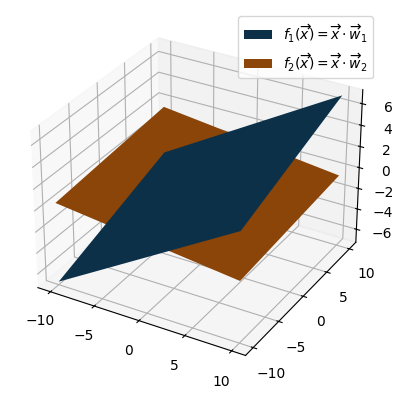
\includegraphics[width=0.5\linewidth]{img/planes.png}
\caption{Planos en $\mathbb{R}^2\to\mathbb{R}$}
\label{fig:planes}
\end{figure}

\item Para cada plano, grafique el vector normal en el punto $P=(1,1)$ y una curva de nivel perpendicular a tal vector normal. Calcule el vector gradiente en tal punto, y demuestre que ese vector gradiente es perpendicular a la curva de nivel previamente dibujada.

\begin{figure}[h]
\centering
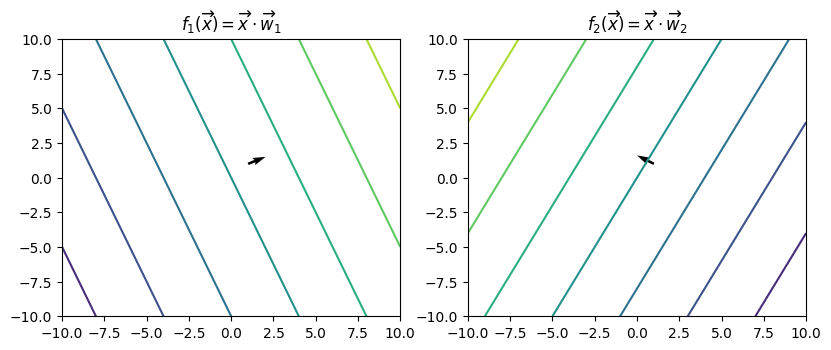
\includegraphics[width=\linewidth]{img/level_curves.png}
\caption{Curvas de nivel y vectores normales.}
\label{fig:level_curves}
\end{figure}

Para demostrar que $\nabla f_1$ es perpendicular a la curva de nivel en $(1,1)$, basta con mostrar que el producto punto entre $\nabla f_1$ y $[1,1,f_1(1,1)]$ da como resultado 0.

\begin{equation}
f_1(\overrightarrow{x})=f_1(x,y)=0.5x+0.2y=z\Rightarrow 0.5x+0.2y-z=0
\end{equation}

\begin{equation}
\begin{array}{rcl}
\nabla f_1\cdot[1,1,f_1(1,1)]&=&\left[\frac{df_1}{dx},\frac{df_1}{dy},\frac{df_1}{dz}\right]\cdot[1,1,0.5+0.2]\\
&=&[0.5,0.2,-1]\cdot[1,1,0.7]\\
&=&0.5\cdot1+0.2\cdot1-1\cdot0.7\\
&=&0
\end{array}
\end{equation}

Para demostrar que $\nabla f_2$ es perpendicular a la curva de nivel en $(1,1)$, basta con mostrar que el producto punto entre $\nabla f_2$ y $[1,1,f_2(1,1)]$ da como resultado 0.

\begin{equation}
f_2(\overrightarrow{x})=f_2(x,y)=-0.1x+0.05y=z\Rightarrow -0.1x+0.05y-z=0
\end{equation}

\begin{equation}
\begin{array}{rcl}
\nabla f_2\cdot[1,1,f_2(1,1)]&=&\left[\frac{df_2}{dx},\frac{df_2}{dy},\frac{df_2}{dz}\right]\cdot[1,1,-0.1+0.05]\\
&=&[-0.1,0.05,-1]\cdot[1,1,-0.05]\\
&=&-0.1\cdot1+0.05\cdot1+1\cdot0.05\\
&=&0
\end{array}
\end{equation}
\end{enumerate}

\subsection{El vector gradiente}

Para cada una de las siguientes funciones multivariable:

\begin{equation}
\begin{array}{l}
f_1(x,y)=(1.5-x+xy)^2+(2.25-x+xy^2)+(2.625-x+xy^3)\\
f_2(x,y)=(x+2y-7)^2+(2x+y-5)^2\\
f_3(x,y)=100\sqrt{|y-0.01x^2|}+0.01|x+10|
\end{array}
\end{equation}

\begin{enumerate}
\item Grafique su superficie con dominio entre -10 y 10.

\begin{figure}[h]
\centering
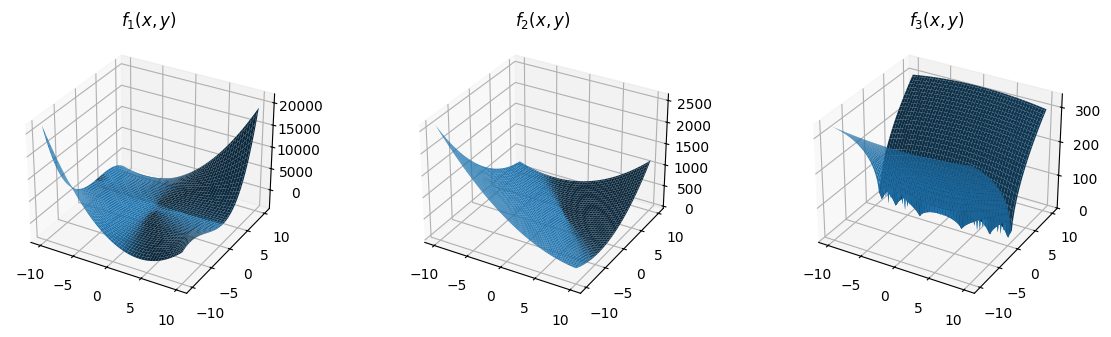
\includegraphics[width=\linewidth]{img/surfaces.png}
\caption{Superficies en el dominio entre -10 y 10.}
\label{fig:surfaces}
\end{figure}

\item Calcule el vector gradiente manualmente, evalúelo y grafique el vector unitario en la dirección del gradiente para los dos puntos especificados (en la misma figura de la superficie).

\begin{equation}
\begin{array}{rcl}
\nabla f_1&=&\left[\frac{df_1}{dx},\frac{df_1}{dy}\right]\\
\frac{df_1}{dx}&=&2(1.5-x+xy)(y-1)+(y^2-1)+(y^3-1)\\
\frac{df_1}{dy}&=&2(1.5-x+xy)x+2xy+3xy^2\\
\nabla f_1(0,0)&=&[-5,0]\\
\nabla f_1(2,2)&=&[17,46]
\end{array}
\end{equation}

\begin{equation}
\begin{array}{rcl}
\nabla f_2&=&\left[\frac{df_2}{dx},\frac{df_2}{dy}\right]\\
\frac{df_2}{dx}&=&2(x+2y-7)+4(2x+y-5)\\
\frac{df_2}{dy}&=&4(x+2y-7)+2(2x+y-5)\\
\nabla f_2(1.5,-5.5)&=&[-63,-81]\\
\nabla f_2(-7,-7)&=&[-160,-164]
\end{array}
\end{equation}

\begin{equation}
\begin{array}{rcl}
\nabla f_3&=&\left[\frac{df_3}{dx},\frac{df_3}{dy}\right]\\
u&=&y-0.01x^2\\
\frac{df_3}{dx}&=&-x\frac{\text{sgn}(u)}{\sqrt{|u|}}+0.01\cdot\text{sgn}(x+10)\\
\frac{df_3}{dy}&=&50\frac{\text{sgn}(u)}{\sqrt{|u|}}\\
\nabla f_3(-4,-2)&\approx&[-2.7117,-34.0207]\\
\nabla f_3(-2,3)&\approx&[1.1725,29.0619]
\end{array}
\end{equation}

\begin{figure}[h]
\centering
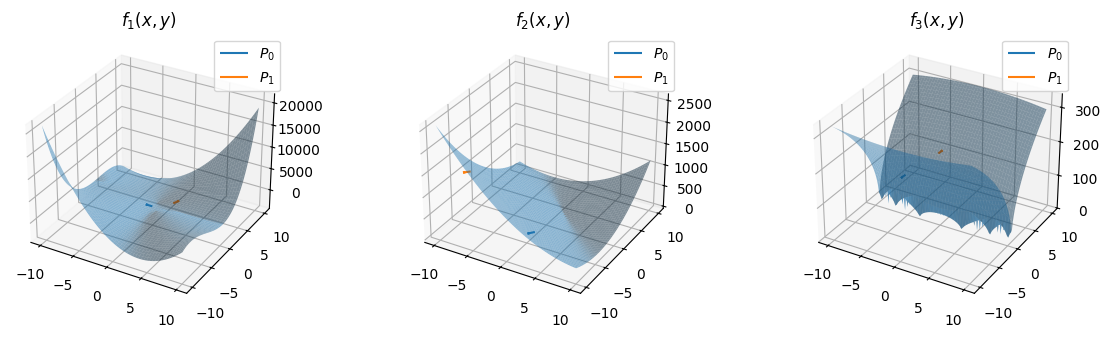
\includegraphics[width=\linewidth]{img/surfaces_quivers.png}
\caption{Superficies con vectores unitarios en la dirección del gradiente para cada punto especificado.}
\label{fig:surfaces_quivers}
\end{figure}

\begin{figure}[h]
\centering
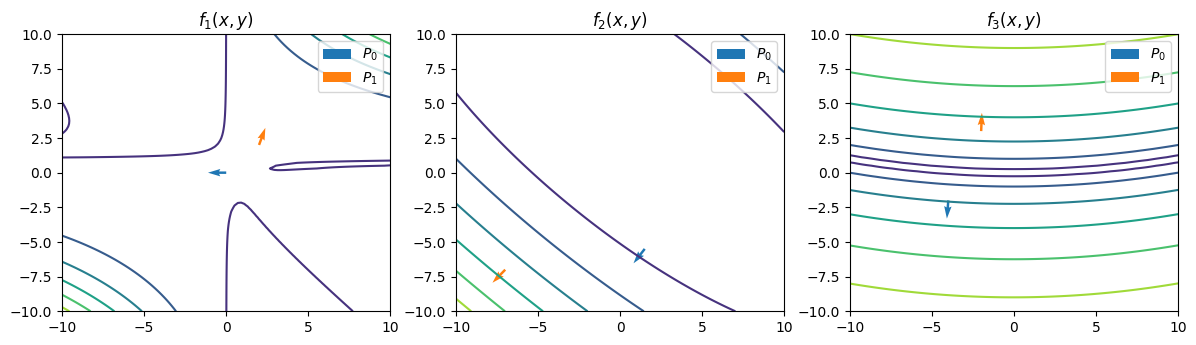
\includegraphics[width=\linewidth]{img/surfaces_level_curves.png}
\caption{Curvas de nivel con vectores unitarios en la dirección del gradiente para cada punto especificado.}
\label{fig:surfaces_level_curves}
\end{figure}

\item Calcule la magnitud de tal vector gradiente en cada punto.

\begin{equation}
\begin{array}{rclll}
||\nabla f_1(0,0)||_2&=&\sqrt{(-5)^2+0^2}&=&5\\
||\nabla f_1(2,2)||_2&=&\sqrt{17^2+46^2}&\approx&49.0408\\
||\nabla f_2(1.5,-5.5)||_2&=&\sqrt{(-63)^2+(-81)^2}&\approx&102.6158\\
||\nabla f_2(-7,-7)||_2&=&\sqrt{(-160)^2+(-164)^2}&\approx&229.1201\\
||\nabla f_3(-4,-2)||_2&\approx&\sqrt{(-2.7117)^2+(-34.0207)^2}&\approx&34.1286\\
||\nabla f_3(-2,3)||_2&\approx&\sqrt{1.1725^2+29.0619^2}&\approx&29.0856
\end{array}
\end{equation}

\item Calcule lo que se conoce como la matriz Hessiana.

\begin{equation}
\begin{array}{rcl}
H_{f(x,y)}&=&
\begin{bmatrix}
\frac{d^2f}{dx^2}&\frac{d^2f}{dxy}\\
\frac{d^2f}{dyx}&\frac{d^2f}{dy^2}
\end{bmatrix}\\
H_{f_1(x,y)}&=&
\begin{bmatrix}
2(y-1)^2&2(1.5-2x+2xy)+2y+3y^2\\
2(1.5-2x+2xy)+2y+3y^2&2x^2+2x+6xy
\end{bmatrix}\\
H_{f_2(x,y)}&=&
\begin{bmatrix}
10&8\\
8&10
\end{bmatrix}\\
u&=&y-0.01x^2\\
H_{f_3(x,y)}&=&
\begin{bmatrix}
\frac{-\text{sgn}(u)}{\sqrt{|u|}}-\frac{0.01x^3}{|u|^{1.5}}&\frac{x}{2|u|^{1.5}}\\
\frac{x}{2|u|^{1.5}}&\frac{-25}{|u|^{1.5}}
\end{bmatrix}\\
\end{array}
\end{equation}
\end{enumerate}

\section{Implementación del algoritmo K-vecinos más cercanos}

El algoritmo de K-vecinos más cercanos es un algoritmo de aprendizaje automático supervisado muy popular por su simplicidad. Dado un conjunto de datos representado matricialmente en la matriz $X_{\textrm{train}}\in\mathbb{R}^{N\times D}$ y un arreglo de etiquetas $\overrightarrow{t}\in\mathbb{R}^{N}$:
\[
X_{\textrm{train}}=\begin{bmatrix}- & \overrightarrow{x}_{1} & -\\
 & \vdots\\
- & \overrightarrow{x}_{N_{\textrm{train}}} & -
\end{bmatrix}\qquad\overrightarrow{t}=\begin{bmatrix}t_{1}\\
\vdots\\
t_{N_{\textrm{train}}}
\end{bmatrix}
\]
Para cada dato $\overrightarrow{x}_{i}^{\left(\textrm{test}\right)}\in X_{\textrm{test}}$ en un conjunto de datos de prueba o evaluación $X_{\textrm{test}}\in\mathbb{R}^{N_{\textrm{test}}\times D}$:
\[
X_{\textrm{test}}=\begin{bmatrix}- & \overrightarrow{x}_{1} & -\\
 & \vdots\\
- & \overrightarrow{x}_{N} & -
\end{bmatrix}
\]
se crea un conjunto de datos $X_{\textrm{KNN}}$ con los $K$ vecinos más cercanos de la observación $\overrightarrow{x}_{j}$ en el conjunto
de datos $X_{\textrm{train}}$, donde cada observación $\overrightarrow{x}_{i}\in X_{\textrm{KNN}}$ cumple que:
\[
X_{\textrm{KNN}}=\arg\min_{K\:\textrm{min}\:j}\left(d\left(\overrightarrow{x}_{i}^{\left(\textrm{test}\right)}-\overrightarrow{x}_{j}\right)\right)
\]

Luego de tomar los K vecinos más cercanos de la observación $\overrightarrow{x}_{i}^{\left(\textrm{test}\right)}$ se realiza una votación según las etiquetas correspondientes $t_{i}^{\left(\textrm{test}\right)}$, y se toma como estimación de la etiqueta $\widetilde{t}_{j}$ la etiqueta
mas votada. 
\begin{enumerate}
\item Implemente el algoritmo de K-vecinos mas cercanos con la posibilidad de usar la distancia euclidiana, de Manhattan, Infinito en la función $d\left(\overrightarrow{x}_{i}-\overrightarrow{x}_{j}\right)$. 
\begin{enumerate}
\item Realice la implementación de forma completamente matricial, para cada observacion $\overrightarrow{x}_{i}^{\left(\textrm{test}\right)}$
\emph{evaluate\_k\_nearest\_neighbors\_observation(data\_training, labels\_training, test\_observation, K = 7, p = 2)} (\textbf{No use
ciclos }\textbf{\emph{for}}).
\begin{enumerate}
\item Para ello use funcionalidades de \emph{pytorch }como \emph{repeat}, \emph{mode}, \emph{sort}, etc. 
\item \emph{p} indica el tipo de norma a utilizar. $K$ corresponde a la cantidad de vecinos a evaluar.
\item Diseñe al menos 2 pruebas unitarias para esta función.

\textbf{Implementación i, ii:}
\begin{tcolorbox}[breakable, size=fbox, boxrule=1pt, pad at break*=1mm,colback=cellbackground, colframe=cellborder]
\prompt{In}{incolor}{ }{\boxspacing}
\begin{Verbatim}[commandchars=\\\{\}]
\PY{c+c1}{\PYZsh{}1.a}
\PY{k}{def}\PY{+w}{ }\PY{n+nf}{evaluate\PYZus{}k\PYZus{}nearest\PYZus{}neighbors\PYZus{}observation}\PY{p}{(}\PY{n}{data\PYZus{}training}\PY{p}{,} \PY{n}{labels\PYZus{}training}\PY{p}{,} \PY{n}{test\PYZus{}observation}\PY{p}{,} \PY{n}{k}\PY{o}{=}\PY{l+m+mi}{7}\PY{p}{,} \PY{n}{p}\PY{o}{=}\PY{l+m+mf}{2.0}\PY{p}{)}\PY{p}{:}

  \PY{c+c1}{\PYZsh{} Calcula la distancia entre la observacion de entrada y el resto del dataset.}
  \PY{k}{if} \PY{n}{p} \PY{o}{==} \PY{n+nb}{float}\PY{p}{(}\PY{l+s+s1}{\PYZsq{}}\PY{l+s+s1}{inf}\PY{l+s+s1}{\PYZsq{}}\PY{p}{)}\PY{p}{:}
    \PY{n}{dist} \PY{o}{=} \PY{n}{torch}\PY{o}{.}\PY{n}{max}\PY{p}{(}\PY{n}{torch}\PY{o}{.}\PY{n}{abs}\PY{p}{(}\PY{n}{data\PYZus{}training} \PY{o}{\PYZhy{}} \PY{n}{test\PYZus{}observation}\PY{p}{)}\PY{p}{,} \PY{n}{dim}\PY{o}{=}\PY{l+m+mi}{1}\PY{p}{)}\PY{o}{.}\PY{n}{values}\PY{o}{.}\PY{n}{unsqueeze}\PY{p}{(}\PY{l+m+mi}{0}\PY{p}{)}
  \PY{k}{else}\PY{p}{:}
    \PY{n}{dist} \PY{o}{=} \PY{n}{torch}\PY{o}{.}\PY{n}{pow}\PY{p}{(}\PY{n}{torch}\PY{o}{.}\PY{n}{sum}\PY{p}{(}\PY{n}{torch}\PY{o}{.}\PY{n}{pow}\PY{p}{(}\PY{n}{torch}\PY{o}{.}\PY{n}{abs}\PY{p}{(}\PY{n}{data\PYZus{}training} \PY{o}{\PYZhy{}} \PY{n}{test\PYZus{}observation}\PY{p}{)}\PY{p}{,} \PY{n}{p}\PY{p}{)}\PY{p}{,} \PY{n}{dim}\PY{o}{=}\PY{l+m+mi}{1}\PY{p}{)}\PY{p}{,} \PY{l+m+mi}{1}\PY{o}{/}\PY{n}{p}\PY{p}{)}\PY{o}{.}\PY{n}{unsqueeze}\PY{p}{(}\PY{l+m+mi}{0}\PY{p}{)}
  
  \PY{c+c1}{\PYZsh{} Se seleccionan los K indices con las menores distancias}
  \PY{n}{k\PYZus{}vecinos} \PY{o}{=} \PY{n}{dist}\PY{o}{.}\PY{n}{topk}\PY{p}{(}\PY{n}{k}\PY{p}{,} \PY{n}{largest}\PY{o}{=}\PY{k+kc}{False}\PY{p}{)}

  \PY{c+c1}{\PYZsh{} Extraccion de los labels de los vecinos mas cercanos}
  \PY{n}{target\PYZus{}labels} \PY{o}{=} \PY{n}{labels\PYZus{}training}\PY{p}{[}\PY{n}{k\PYZus{}vecinos}\PY{o}{.}\PY{n}{indices}\PY{p}{[}\PY{l+m+mi}{0}\PY{p}{]}\PY{p}{]}

  \PY{c+c1}{\PYZsh{} La moda se puede usar para obtener el valor más repetido}
  \PY{c+c1}{\PYZsh{} Este valor se convierte en la etiqueta estimada}
  \PY{k}{return} \PY{n}{torch}\PY{o}{.}\PY{n}{mode}\PY{p}{(}\PY{n}{target\PYZus{}labels}\PY{p}{,} \PY{l+m+mi}{0}\PY{p}{)}\PY{o}{.}\PY{n}{values}\PY{o}{.}\PY{n}{unsqueeze}\PY{p}{(}\PY{l+m+mi}{0}\PY{p}{)}
\end{Verbatim}
\end{tcolorbox}

\textbf{Pruebas Unitarias iii:}

\begin{tcolorbox}[breakable, size=fbox, boxrule=1pt, pad at break*=1mm,colback=cellbackground, colframe=cellborder]
\prompt{In}{incolor}{ }{\boxspacing}
\begin{Verbatim}[commandchars=\\\{\}]
\PY{c+c1}{\PYZsh{} Datos de prueba}
\PY{n}{ut\PYZus{}data} \PY{o}{=} \PY{n}{torch}\PY{o}{.}\PY{n}{tensor}\PY{p}{(}\PY{p}{[}\PY{p}{[}\PY{l+m+mf}{1.0}\PY{p}{,} \PY{l+m+mf}{2.0}\PY{p}{]}\PY{p}{,} \PY{p}{[}\PY{l+m+mf}{2.0}\PY{p}{,} \PY{l+m+mf}{3.0}\PY{p}{]}\PY{p}{,} \PY{p}{[}\PY{l+m+mf}{3.0}\PY{p}{,} \PY{l+m+mf}{4.0}\PY{p}{]}\PY{p}{,} \PY{p}{[}\PY{l+m+mf}{6.0}\PY{p}{,} \PY{l+m+mf}{7.0}\PY{p}{]}\PY{p}{,} \PY{p}{[}\PY{l+m+mf}{7.0}\PY{p}{,} \PY{l+m+mf}{8.0}\PY{p}{]}\PY{p}{]}\PY{p}{)}
\PY{n}{ut\PYZus{}labels} \PY{o}{=} \PY{n}{torch}\PY{o}{.}\PY{n}{tensor}\PY{p}{(}\PY{p}{[}\PY{l+m+mi}{0}\PY{p}{,} \PY{l+m+mi}{0}\PY{p}{,} \PY{l+m+mi}{0}\PY{p}{,} \PY{l+m+mi}{1}\PY{p}{,} \PY{l+m+mi}{1}\PY{p}{]}\PY{p}{)}\PY{o}{.}\PY{n}{unsqueeze}\PY{p}{(}\PY{l+m+mi}{1}\PY{p}{)}  \PY{c+c1}{\PYZsh{} Dos clases: 0 y 1}

\PY{c+c1}{\PYZsh{}Puntos a evaluar}
\PY{n}{punto1} \PY{o}{=} \PY{n}{torch}\PY{o}{.}\PY{n}{tensor}\PY{p}{(}\PY{p}{[}\PY{l+m+mf}{2.5}\PY{p}{,} \PY{l+m+mf}{3.5}\PY{p}{]}\PY{p}{)} \PY{c+c1}{\PYZsh{} clase 0}
\PY{n}{punto2} \PY{o}{=} \PY{n}{torch}\PY{o}{.}\PY{n}{tensor}\PY{p}{(}\PY{p}{[}\PY{l+m+mf}{5.5}\PY{p}{,} \PY{l+m+mf}{6.5}\PY{p}{]}\PY{p}{)} \PY{c+c1}{\PYZsh{} clase 1}
\PY{n}{punto3} \PY{o}{=} \PY{n}{torch}\PY{o}{.}\PY{n}{tensor}\PY{p}{(}\PY{p}{[}\PY{l+m+mf}{1.5}\PY{p}{,} \PY{l+m+mf}{2.5}\PY{p}{]}\PY{p}{)} \PY{c+c1}{\PYZsh{} clase 0}

\PY{n+nb}{print}\PY{p}{(}\PY{l+s+sa}{f}\PY{l+s+s1}{\PYZsq{}}\PY{l+s+s1}{ut\PYZus{}data shape:}\PY{l+s+se}{\PYZbs{}t}\PY{l+s+se}{\PYZbs{}t}\PY{l+s+si}{\PYZob{}}\PY{n}{ut\PYZus{}data}\PY{o}{.}\PY{n}{shape}\PY{l+s+si}{\PYZcb{}}\PY{l+s+se}{\PYZbs{}n}\PY{l+s+s1}{ut\PYZus{}labels shape:}\PY{l+s+se}{\PYZbs{}t}\PY{l+s+si}{\PYZob{}}\PY{n}{ut\PYZus{}labels}\PY{o}{.}\PY{n}{shape}\PY{l+s+si}{\PYZcb{}}\PY{l+s+s1}{\PYZsq{}}\PY{p}{)}

\PY{c+c1}{\PYZsh{} Plotting datos de prueba}
\PY{n}{plt}\PY{o}{.}\PY{n}{scatter}\PY{p}{(}\PY{n}{ut\PYZus{}data}\PY{p}{[}\PY{p}{:}\PY{p}{,} \PY{l+m+mi}{0}\PY{p}{]}\PY{p}{,} \PY{n}{ut\PYZus{}data}\PY{p}{[}\PY{p}{:}\PY{p}{,} \PY{l+m+mi}{1}\PY{p}{]}\PY{p}{,} \PY{n}{c}\PY{o}{=}\PY{n}{ut\PYZus{}labels}\PY{o}{.}\PY{n}{squeeze}\PY{p}{(}\PY{p}{)}\PY{p}{)}

\PY{c+c1}{\PYZsh{} Plotting puntos especificos de pruebas}
\PY{n}{plt}\PY{o}{.}\PY{n}{scatter}\PY{p}{(}\PY{n}{punto1}\PY{p}{[}\PY{l+m+mi}{0}\PY{p}{]}\PY{p}{,} \PY{n}{punto1}\PY{p}{[}\PY{l+m+mi}{1}\PY{p}{]}\PY{p}{,} \PY{n}{color}\PY{o}{=}\PY{l+s+s1}{\PYZsq{}}\PY{l+s+s1}{red}\PY{l+s+s1}{\PYZsq{}}\PY{p}{,} \PY{n}{marker}\PY{o}{=}\PY{l+s+s1}{\PYZsq{}}\PY{l+s+s1}{x}\PY{l+s+s1}{\PYZsq{}}\PY{p}{,} \PY{n}{label}\PY{o}{=}\PY{l+s+s1}{\PYZsq{}}\PY{l+s+s1}{Punto de prueba 1}\PY{l+s+s1}{\PYZsq{}}\PY{p}{)}
\PY{n}{plt}\PY{o}{.}\PY{n}{scatter}\PY{p}{(}\PY{n}{punto2}\PY{p}{[}\PY{l+m+mi}{0}\PY{p}{]}\PY{p}{,} \PY{n}{punto2}\PY{p}{[}\PY{l+m+mi}{1}\PY{p}{]}\PY{p}{,} \PY{n}{color}\PY{o}{=}\PY{l+s+s1}{\PYZsq{}}\PY{l+s+s1}{green}\PY{l+s+s1}{\PYZsq{}}\PY{p}{,} \PY{n}{marker}\PY{o}{=}\PY{l+s+s1}{\PYZsq{}}\PY{l+s+s1}{x}\PY{l+s+s1}{\PYZsq{}}\PY{p}{,} \PY{n}{label}\PY{o}{=}\PY{l+s+s1}{\PYZsq{}}\PY{l+s+s1}{Punto de prueba 2}\PY{l+s+s1}{\PYZsq{}}\PY{p}{)}
\PY{n}{plt}\PY{o}{.}\PY{n}{scatter}\PY{p}{(}\PY{n}{punto3}\PY{p}{[}\PY{l+m+mi}{0}\PY{p}{]}\PY{p}{,} \PY{n}{punto3}\PY{p}{[}\PY{l+m+mi}{1}\PY{p}{]}\PY{p}{,} \PY{n}{color}\PY{o}{=}\PY{l+s+s1}{\PYZsq{}}\PY{l+s+s1}{blue}\PY{l+s+s1}{\PYZsq{}}\PY{p}{,} \PY{n}{marker}\PY{o}{=}\PY{l+s+s1}{\PYZsq{}}\PY{l+s+s1}{x}\PY{l+s+s1}{\PYZsq{}}\PY{p}{,} \PY{n}{label}\PY{o}{=}\PY{l+s+s1}{\PYZsq{}}\PY{l+s+s1}{Punto de prueba 3}\PY{l+s+s1}{\PYZsq{}}\PY{p}{)}

\PY{n}{plt}\PY{o}{.}\PY{n}{xlabel}\PY{p}{(}\PY{l+s+s1}{\PYZsq{}}\PY{l+s+s1}{Feature 1}\PY{l+s+s1}{\PYZsq{}}\PY{p}{)}
\PY{n}{plt}\PY{o}{.}\PY{n}{ylabel}\PY{p}{(}\PY{l+s+s1}{\PYZsq{}}\PY{l+s+s1}{Feature 2}\PY{l+s+s1}{\PYZsq{}}\PY{p}{)}
\PY{n}{plt}\PY{o}{.}\PY{n}{title}\PY{p}{(}\PY{l+s+s1}{\PYZsq{}}\PY{l+s+s1}{Observaciones para unit tests}\PY{l+s+s1}{\PYZsq{}}\PY{p}{)}
\PY{n}{plt}\PY{o}{.}\PY{n}{legend}\PY{p}{(}\PY{p}{)}
\PY{n}{plt}\PY{o}{.}\PY{n}{show}\PY{p}{(}\PY{p}{)}
\end{Verbatim}
\end{tcolorbox}

    \begin{Verbatim}[commandchars=\\\{\}]
ut\_data shape:          torch.Size([5, 2])
ut\_labels shape:        torch.Size([5, 1])
    \end{Verbatim}

    \begin{figure}
    \centering
    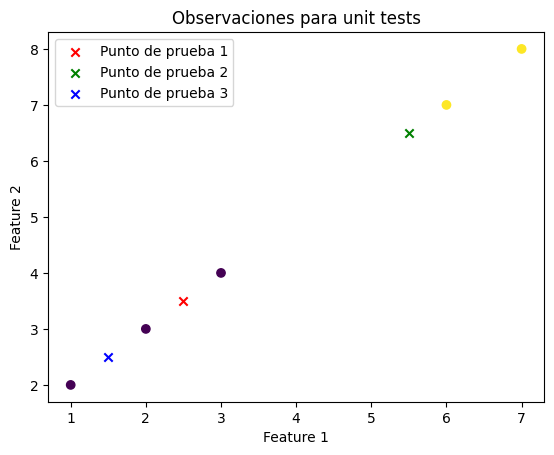
\includegraphics[width=0.5\linewidth]{img/output_39_1.png}
    \caption{Dataset de pruebas unitarias con 5 observaciones, 3 de clase 0 y 2 de clase 1. Las $x$ muestran los puntos de prueba (pivote) para probar el algoritmo de KNN.}
    \label{fig:ut_dataset}    
\end{figure}

    
    \begin{tcolorbox}[breakable, size=fbox, boxrule=1pt, pad at break*=1mm,colback=cellbackground, colframe=cellborder]
\prompt{In}{incolor}{ }{\boxspacing}
\begin{Verbatim}[commandchars=\\\{\}]
\PY{c+c1}{\PYZsh{} Test bench}

\PY{k}{def}\PY{+w}{ }\PY{n+nf}{ut\PYZus{}p}\PY{p}{(}\PY{n}{test\PYZus{}point}\PY{p}{,} \PY{n}{expected\PYZus{}class}\PY{p}{,} \PY{n}{p}\PY{p}{)}\PY{p}{:}
  \PY{n}{test\PYZus{}estimations\PYZus{}all} \PY{o}{=} \PY{n}{evaluate\PYZus{}k\PYZus{}nearest\PYZus{}neighbors\PYZus{}observation}\PY{p}{(}\PY{n}{ut\PYZus{}data}\PY{p}{,} \PY{n}{ut\PYZus{}labels}\PY{p}{,} \PY{n}{test\PYZus{}point}\PY{p}{,} \PY{n}{k} \PY{o}{=} \PY{l+m+mi}{2}\PY{p}{,} \PY{n}{p}\PY{o}{=}\PY{n}{p}\PY{p}{,} \PY{n}{debug}\PY{o}{=}\PY{k+kc}{True}\PY{p}{)}
  \PY{n+nb}{print}\PY{p}{(}\PY{l+s+s2}{\PYZdq{}}\PY{l+s+s2}{Clase estimada: }\PY{l+s+s2}{\PYZdq{}}\PY{p}{,} \PY{n}{test\PYZus{}estimations\PYZus{}all}\PY{o}{.}\PY{n}{squeeze}\PY{p}{(}\PY{l+m+mi}{1}\PY{p}{)}\PY{p}{)}
  \PY{n+nb}{print}\PY{p}{(}\PY{l+s+s2}{\PYZdq{}}\PY{l+s+s2}{Clase esperada: }\PY{l+s+s2}{\PYZdq{}}\PY{p}{,} \PY{n}{torch}\PY{o}{.}\PY{n}{tensor}\PY{p}{(}\PY{p}{[}\PY{l+m+mi}{0}\PY{p}{]}\PY{p}{)}\PY{p}{)}
  \PY{k}{if} \PY{n}{torch}\PY{o}{.}\PY{n}{equal}\PY{p}{(}\PY{n}{test\PYZus{}estimations\PYZus{}all}\PY{o}{.}\PY{n}{squeeze}\PY{p}{(}\PY{l+m+mi}{1}\PY{p}{)}\PY{p}{,} \PY{n}{expected\PYZus{}class}\PY{p}{)}\PY{p}{:}
    \PY{n+nb}{print}\PY{p}{(}\PY{l+s+sa}{f}\PY{l+s+s2}{\PYZdq{}}\PY{l+s+s2}{Test }\PY{l+s+si}{\PYZob{}}\PY{n}{p}\PY{l+s+si}{\PYZcb{}}\PY{l+s+s2}{ passed}\PY{l+s+s2}{\PYZdq{}}\PY{p}{)}
    \PY{k}{return} \PY{k+kc}{True}

  \PY{n+nb}{print}\PY{p}{(}\PY{l+s+sa}{f}\PY{l+s+s2}{\PYZdq{}}\PY{l+s+s2}{Test }\PY{l+s+si}{\PYZob{}}\PY{n}{p}\PY{l+s+si}{\PYZcb{}}\PY{l+s+s2}{ failed}\PY{l+s+s2}{\PYZdq{}}\PY{p}{)}
  \PY{k}{return} \PY{k+kc}{False}
\end{Verbatim}
\end{tcolorbox}

    \textbf{Ejecución de pruebas}

    \begin{tcolorbox}[breakable, size=fbox, boxrule=1pt, pad at break*=1mm,colback=cellbackground, colframe=cellborder]
\prompt{In}{incolor}{ }{\boxspacing}
\begin{Verbatim}[commandchars=\\\{\}]
\PY{n}{pruebas} \PY{o}{=} \PY{p}{[}\PY{p}{]}
\PY{n+nb}{print}\PY{p}{(}\PY{l+s+s2}{\PYZdq{}}\PY{l+s+s2}{Unit test 1}\PY{l+s+s2}{\PYZdq{}}\PY{p}{)}
\PY{n}{pruebas}\PY{o}{.}\PY{n}{append}\PY{p}{(}\PY{n}{ut\PYZus{}p}\PY{p}{(}\PY{n}{punto1}\PY{p}{,} \PY{n}{torch}\PY{o}{.}\PY{n}{tensor}\PY{p}{(}\PY{p}{[}\PY{l+m+mi}{0}\PY{p}{]}\PY{p}{)}\PY{p}{,} \PY{l+m+mf}{1.0}\PY{p}{)}\PY{p}{)}
\PY{n+nb}{print}\PY{p}{(}\PY{l+s+s2}{\PYZdq{}}\PY{l+s+s2}{Unit test 2}\PY{l+s+s2}{\PYZdq{}}\PY{p}{)}
\PY{n}{pruebas}\PY{o}{.}\PY{n}{append}\PY{p}{(}\PY{n}{ut\PYZus{}p}\PY{p}{(}\PY{n}{punto2}\PY{p}{,} \PY{n}{torch}\PY{o}{.}\PY{n}{tensor}\PY{p}{(}\PY{p}{[}\PY{l+m+mi}{1}\PY{p}{]}\PY{p}{)}\PY{p}{,} \PY{l+m+mf}{1.0}\PY{p}{)}\PY{p}{)}
\PY{n+nb}{print}\PY{p}{(}\PY{l+s+s2}{\PYZdq{}}\PY{l+s+s2}{Unit test 3}\PY{l+s+s2}{\PYZdq{}}\PY{p}{)}
\PY{n}{pruebas}\PY{o}{.}\PY{n}{append}\PY{p}{(}\PY{n}{ut\PYZus{}p}\PY{p}{(}\PY{n}{punto3}\PY{p}{,} \PY{n}{torch}\PY{o}{.}\PY{n}{tensor}\PY{p}{(}\PY{p}{[}\PY{l+m+mi}{0}\PY{p}{]}\PY{p}{)}\PY{p}{,} \PY{l+m+mf}{1.0}\PY{p}{)}\PY{p}{)}
\end{Verbatim}
\end{tcolorbox}

    \begin{Verbatim}[commandchars=\\\{\}]
Prueba      Passed
 Prueba 1    True
 Prueba 2    True
 Prueba 3    True
    \end{Verbatim}


\end{enumerate}
\item Para todo el conjunto de datos $X_{\textrm{test}}$ implemente la funcion \emph{evaluate\_k\_nearest\_neighbors\_test\_dataset(data\_training, labels\_training, test\_dataset, K = 3, is\_euclidian = True), }la cual utilice la función previamente construida \emph{evaluate\_k\_nearest\_neighbors\_observation} para calcular el arreglo de estimaciones $\overrightarrow{\widetilde{t}}$
para todos los datos en $X_{\textrm{test}}$.

\begin{tcolorbox}[breakable, size=fbox, boxrule=1pt, pad at break*=1mm,colback=cellbackground, colframe=cellborder]
\prompt{In}{incolor}{ }{\boxspacing}
\begin{Verbatim}[commandchars=\\\{\}]
\PY{c+c1}{\PYZsh{}1.b}
\PY{k}{def}\PY{+w}{ }\PY{n+nf}{evaluate\PYZus{}k\PYZus{}nearest\PYZus{}neighbors\PYZus{}test\PYZus{}dataset}\PY{p}{(}\PY{n}{data\PYZus{}training}\PY{p}{,} \PY{n}{labels\PYZus{}training}\PY{p}{,} \PY{n}{test\PYZus{}dataset}\PY{p}{,} \PY{n}{k}\PY{o}{=}\PY{l+m+mi}{3}\PY{p}{,} \PY{n}{p}\PY{o}{=}\PY{n+nb}{float}\PY{p}{(}\PY{l+s+s1}{\PYZsq{}}\PY{l+s+s1}{inf}\PY{l+s+s1}{\PYZsq{}}\PY{p}{)}\PY{p}{)}\PY{p}{:}
\PY{+w}{  }\PY{l+s+sd}{\PYZdq{}\PYZdq{}\PYZdq{}}
\PY{l+s+sd}{  Se elimina la variable de la especificacion is\PYZus{}euclidean, pues se deben soportar tres normas:}
\PY{l+s+sd}{  p = [1, 2, float(\PYZsq{}inf\PYZsq{})]}
\PY{l+s+sd}{  \PYZdq{}\PYZdq{}\PYZdq{}}
  \PY{c+c1}{\PYZsh{} calcula el knn para cada observacion del test\PYZus{}dataset}
  \PY{n}{t\PYZus{}estimated\PYZus{}dataset} \PY{o}{=} \PY{p}{[}
    \PY{n}{evaluate\PYZus{}k\PYZus{}nearest\PYZus{}neighbors\PYZus{}observation}\PY{p}{(}\PY{n}{data\PYZus{}training}\PY{p}{,} \PY{n}{labels\PYZus{}training}\PY{p}{,} \PY{n}{test\PYZus{}observation}\PY{p}{,} \PY{n}{k}\PY{p}{,} \PY{n}{p}\PY{p}{)}
      \PY{k}{for} \PY{n}{test\PYZus{}observation} \PY{o+ow}{in} \PY{n}{test\PYZus{}dataset}
    \PY{p}{]}

  \PY{c+c1}{\PYZsh{} retorna un tensor en la misma arquitectura que el tensor de data\PYZus{}training}
  \PY{k}{return} \PY{n}{torch}\PY{o}{.}\PY{n}{tensor}\PY{p}{(}\PY{n}{t\PYZus{}estimated\PYZus{}dataset}\PY{p}{)}\PY{o}{.}\PY{n}{to}\PY{p}{(}\PY{n}{data\PYZus{}training}\PY{o}{.}\PY{n}{device}\PY{p}{)}
\end{Verbatim}
\end{tcolorbox}

\item Implemente la función \emph{calcular\_tasa\_aciertos }la cual tome un arreglo de estimaciones $\overrightarrow{\widetilde{t}}$ y un arreglo de etiquetas $\overrightarrow{x}_{i}^{\left(\textrm{test}\right)}$ y calcule la tasa de aciertos definida como $\frac{c}{N}$ donde $c$ es la cantidad de estimaciones correctas. \textbf{(No use ciclos }\textbf{\emph{for}}\textbf{)}.

\begin{tcolorbox}[breakable, size=fbox, boxrule=1pt, pad at break*=1mm,colback=cellbackground, colframe=cellborder]
\prompt{In}{incolor}{ }{\boxspacing}
\begin{Verbatim}[commandchars=\\\{\}]
\PY{c+c1}{\PYZsh{}1.c}
\PY{k}{def}\PY{+w}{ }\PY{n+nf}{calcular\PYZus{}tasa\PYZus{}aciertos}\PY{p}{(}\PY{n}{test\PYZus{}estimations}\PY{p}{,} \PY{n}{test\PYZus{}labels}\PY{p}{)}\PY{p}{:}
\PY{+w}{  }\PY{l+s+sd}{\PYZdq{}\PYZdq{}\PYZdq{} Calcula la tasa de aciertos \PYZdq{}\PYZdq{}\PYZdq{}}
  \PY{n}{comparison} \PY{o}{=} \PY{n}{torch}\PY{o}{.}\PY{n}{eq}\PY{p}{(}\PY{n}{test\PYZus{}estimations}\PY{p}{,} \PY{n}{test\PYZus{}labels}\PY{p}{)}
  \PY{k}{return} \PY{n}{torch}\PY{o}{.}\PY{n}{count\PYZus{}nonzero}\PY{p}{(}\PY{n}{comparison}\PY{p}{,} \PY{n}{dim}\PY{o}{=}\PY{l+m+mi}{0}\PY{p}{)}\PY{o}{.}\PY{n}{item}\PY{p}{(}\PY{p}{)} \PY{o}{/} \PY{n}{test\PYZus{}labels}\PY{o}{.}\PY{n}{shape}\PY{p}{[}\PY{l+m+mi}{0}\PY{p}{]}
\end{Verbatim}
\end{tcolorbox}


\end{enumerate}
\item Para un conjunto de datos de $N=1000000$ (500000 observaciones por clase)\footnote{Se utilizaron un total de $100000$ observaciones, $50000$ por clase, después de consultarlo con el profesor.} genere un conjunto de datos con medias $\mu_{1}=\left[12,12\right]^{T}$, $\mu_{2}=\left[20,20\right]^{T}$, y desviaciones estándar $\sigma_{1}=\left[3,3\right]^{T}$, $\sigma_{2}=\left[2,2\right]^{T}$. Grafique los datos y muestre las figuras.

\begin{figure}
    \centering
    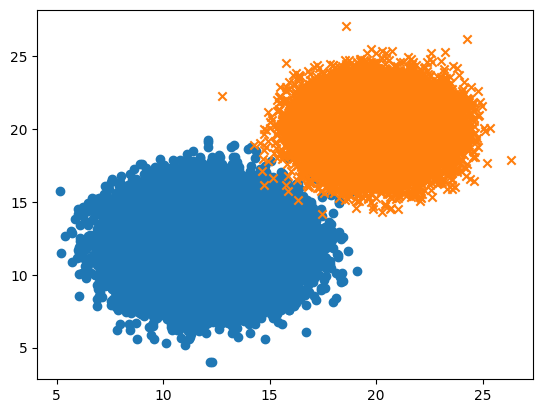
\includegraphics[width=0.5\linewidth]{img/output_49_0.png}
    \caption{Dataset de prueba con cien mil observaciones, 50\% para cada clase: clase 0 azul $\mu_{1}=\left[12,12\right]^{T}$ y $\sigma_{1}=\left[3,3\right]^{T}$, clase 1 naranja $\mu_{2}=\left[20,20\right]^{T}$ y $\sigma_{2}=\left[2,2\right]^{T}$.}
    \label{fig:dataset100k}    
\end{figure}

% { \hspace*{\fill} \\}
\vspace{0.5cm}

\item Compruebe y compare para las tres distancias implementadas, usando el dataset anterior, y $K=7$:
\begin{enumerate}
\item La tasa de aciertos, definida como $\frac{c}{N}$ donde $c$ es la cantidad de estimaciones correctas, usando el mismo conjunto de datos $X_{\textrm{train}}$ como conjunto de prueba $X_{\textrm{test}}$.
Documente los resultados y coméntelos. Puede probar otros valores de medias que faciliten la separabilidad de los datos para facilitar la explicación. 

\begin{table}[H]
    \centering
    \begin{tabular}{c|c}    
        \textbf{Distancia} & \textbf{Tasa de Aciertos} \\
        \hline        
        $\ell_{1}$ &  0.99978\\
        $\ell_{2}$ &  0.99979\\
        $\ell_{\infty}$ &  0.99982\\
    \end{tabular}    
    \caption{\centering \small Tasa de aciertos del algoritmo KNN aplicado a todo el conjunto de datos, utilizando $K=7$, y las tres distancias $\ell_{1}$,$\ell_{2}$ y $\ell_{\infty}$, la tabla muestra los resultados de 1 corrida para cada distancia.}
    \label{tab:resultados_knn_dateset_completo}
\end{table}

\begin{quote}
\textbf{Comentario}: Las tres distancias parecen generar una tasa muy alta de aciertos, las cuales son muy similares entre sí. Esto puede deberse a que si se ve la distribución de las clases en la \textbf{Figura} \ref{fig:dataset100k}, se puede ver que hay poco traslape entre ellas, por lo que el algoritmo, sin importar la distancia utilizada, hace una clasificación efectiva. El hecho de que en ninguna ocasión se obtuvo una tasa de aciertos del $100\%$, es positivo, pues algunas pocas observaciones no son fácilmente clasificables, pues se encuentran traslapadas por completo.
\end{quote}

\vspace{0.5cm}

\item Usando las funciones de partición de datos del paquete \emph{sklearn} necesarias, implemente la partición de datos del conjunto de datos original $X$ para crear las particiones $X_{\textrm{train}}$ y $X_{\textrm{test}}$. Cree 10 particiones distintas, para ejecutar 10 veces el código. 
\begin{enumerate}
\item Utilice 70\% de los datos para entrenamiento y el resto para prueba.
\item Calcule la tasa de aciertos para las 3 configuraciones (distancia $\ell_{1}$,$\ell_{2}$ y $\ell_{\infty}$) probadas, usando $X_{\textrm{train}}$
para entrenamiento y $X_{\textrm{test}}$ para prueba. Reporte los resultados en una tabla, junto con su media y desviación estándar y coméntelos.

\begin{table}[H]
    \centering
\begin{tabular}{r|rrrrrr}
    \toprule
    \multicolumn{7}{c}{\textbf{Tasa de Aciertos}}\\    
    & \multicolumn{2}{c}{Manhattan} & \multicolumn{2}{c}{Euclidean} & \multicolumn{2}{c}{Infinity} \\
    Corrida & GPU & CPU & GPU & CPU & GPU & CPU \\
    \midrule
    1 & 0.999800 & 0.999767 & 0.999800 & 0.999800 & 0.999767 & 0.999733 \\
    2 & 0.999900 & 0.999833 & 0.999867 & 0.999833 & 0.999867 & 0.999800 \\
    3 & 0.999667 & 0.999833 & 0.999700 & 0.999800 & 0.999733 & 0.999767 \\
    4 & 0.999833 & 0.999800 & 0.999833 & 0.999767 & 0.999833 & 0.999733 \\
    5 & 0.999700 & 0.999733 & 0.999733 & 0.999733 & 0.999667 & 0.999733 \\
    6 & 0.999800 & 0.999600 & 0.999800 & 0.999633 & 0.999800 & 0.999667 \\
    7 & 0.999700 & 0.999833 & 0.999700 & 0.999800 & 0.999700 & 0.999800 \\
    8 & 0.999867 & 0.999767 & 0.999833 & 0.999800 & 0.999800 & 0.999800 \\
    9 & 0.999800 & 0.999700 & 0.999833 & 0.999700 & 0.999833 & 0.999700 \\
    10 & 0.999833& 0.999667 & 0.999833 & 0.999633 & 0.999833 & 0.999600 \\
    \midrule
    \textbf{Media}    & \textbf{0.999790} & \textbf{0.999753} & \textbf{0.999793} & \textbf{0.999750} & \textbf{0.999783} & \textbf{0.999733} \\
    \textbf{St. dev.} & \textbf{0.000077} & \textbf{0.000079} & \textbf{0.000060} & \textbf{0.000072} & \textbf{0.000065} & \textbf{0.000065} \\
    \bottomrule
\end{tabular}
\caption{Tasa de aciertos de 10 corridas en GPU con las tres distancias implementadas. Las pruebas se efectuaron en ambientes de Google Colab, utilizando un GPU  A100, mientras que el CPU utilizado fue el provisto en la instancia L4 (alta memoria). Todas las corridas en GPU y CPU utilizaron semillas aleatorias diferentes.}
\label{tab:resultados_10_corridas_gpu_vs_cpu}
\end{table}

\begin{quote}
\textbf{Comentario}: Las tres distancias mantienen la tendencia vista anteriormente en la tabla \ref{tab:resultados_knn_dateset_completo}, donde todas las distancias presentan una tasa muy alta de aciertos, en este caso con una baja desviación estándar, lo cual parece indicar que el KNN presenta casi los mismos resultados sin importar la distancia utilizada. No parece existir una diferencia significativa entre los resultados de GPU y CPU.
\end{quote}

\vspace{0.3cm}

\item Calcule además el \textbf{tiempo de ejecución} por corrida para cada las tres distancias tanto en CPU como en GPU. Reporte los resultados en una tabla para las 10 corridas, junto con su media y desviación estándar y coméntelos. 

\begin{table}[H]
    \centering
    \begin{tabular}{r|rrrrrr}
    \toprule
    \multicolumn{7}{c}{\textbf{Duración en segundos}}\\
    \toprule
    & \multicolumn{2}{c}{Manhattan} & \multicolumn{2}{c}{Euclidean} & \multicolumn{2}{c}{Infinity} \\
    Corrida & GPU & CPU & GPU & CPU & GPU & CPU \\
    \midrule
    1 & 8.086052 & 21.610155 & 7.471702 & 24.006129 & 6.696899 & 18.805519 \\
    2 & 8.071934 & 20.520020 & 7.450645 & 24.019213 & 6.677324 & 18.755920 \\
    3 & 8.194681 & 20.791444 & 7.468749 & 24.013317 & 6.674734 &  18.379076 \\
    4 & 8.067917 & 20.350141 & 7.519531 & 23.636163 & 6.690659 &  18.966814 \\
    5 & 8.088926 & 20.234142 & 7.452440 & 24.011520 & 6.705777 &  19.095105 \\
    6 & 8.115149 & 20.754730 & 7.476169 & 24.103350 & 6.715930 &  18.729428 \\
    7 & 8.072658 & 20.381359 & 7.662809 & 23.968350 & 6.503448 &  19.104312 \\
    8 & 8.052628 & 20.497603 & 7.686365 & 23.902102 & 6.516738 & 18.150882 \\
    9 & 8.092654 & 20.341320 & 7.627234 & 23.946782 & 6.501912 &  18.267952 \\
    10 & 8.062700& 20.645990 & 7.618219 & 23.823238 & 6.699250 &  18.936353 \\
    \midrule
    \textbf{Media}    & \textbf{8.090530} & 20.612691 & \textbf{7.543386} & 23.943016 & \textbf{6.638267} &  18.719136 \\
    \textbf{St. dev.} & \textbf{0.040645} & 0.395726 & \textbf{0.094283} & 0.131642 & \textbf{0.091217} &  0.341449 \\
    \bottomrule
    \end{tabular}
    \caption{Duración en segundos de 10 corridas tanto en GPU como en CPU, con sus medias y desviaciones estándar. Las pruebas se efectuaron en ambientes de Google Colab, utilizando un GPU  A100, mientras que el CPU utilizado fue el provisto en la instancia L4 (alta memoria). Todas las corridas en GPU y CPU utilizaron semillas aleatorias diferentes.}
    \label{tab:duracion_10_corridas_gpu_vs_cpu}
\end{table}

\begin{quote}
    \textbf{Comentario:} El KNN en GPU parece ser más rápido que en CPU, por al menos 1 orden de magnitud. Para todas las distancias utilizadas, los resultados en GPU son superiores, lo cual es consecuente con la implementación matricial del algoritmo KNN y  el hecho que los GPUs pueden realizar operaciones matriciales de forma más eficiente y paralela que en CPU.
\end{quote}
\newpage
\begin{enumerate}
\item Realice una gráfica comparativa.

\begin{figure}
    
    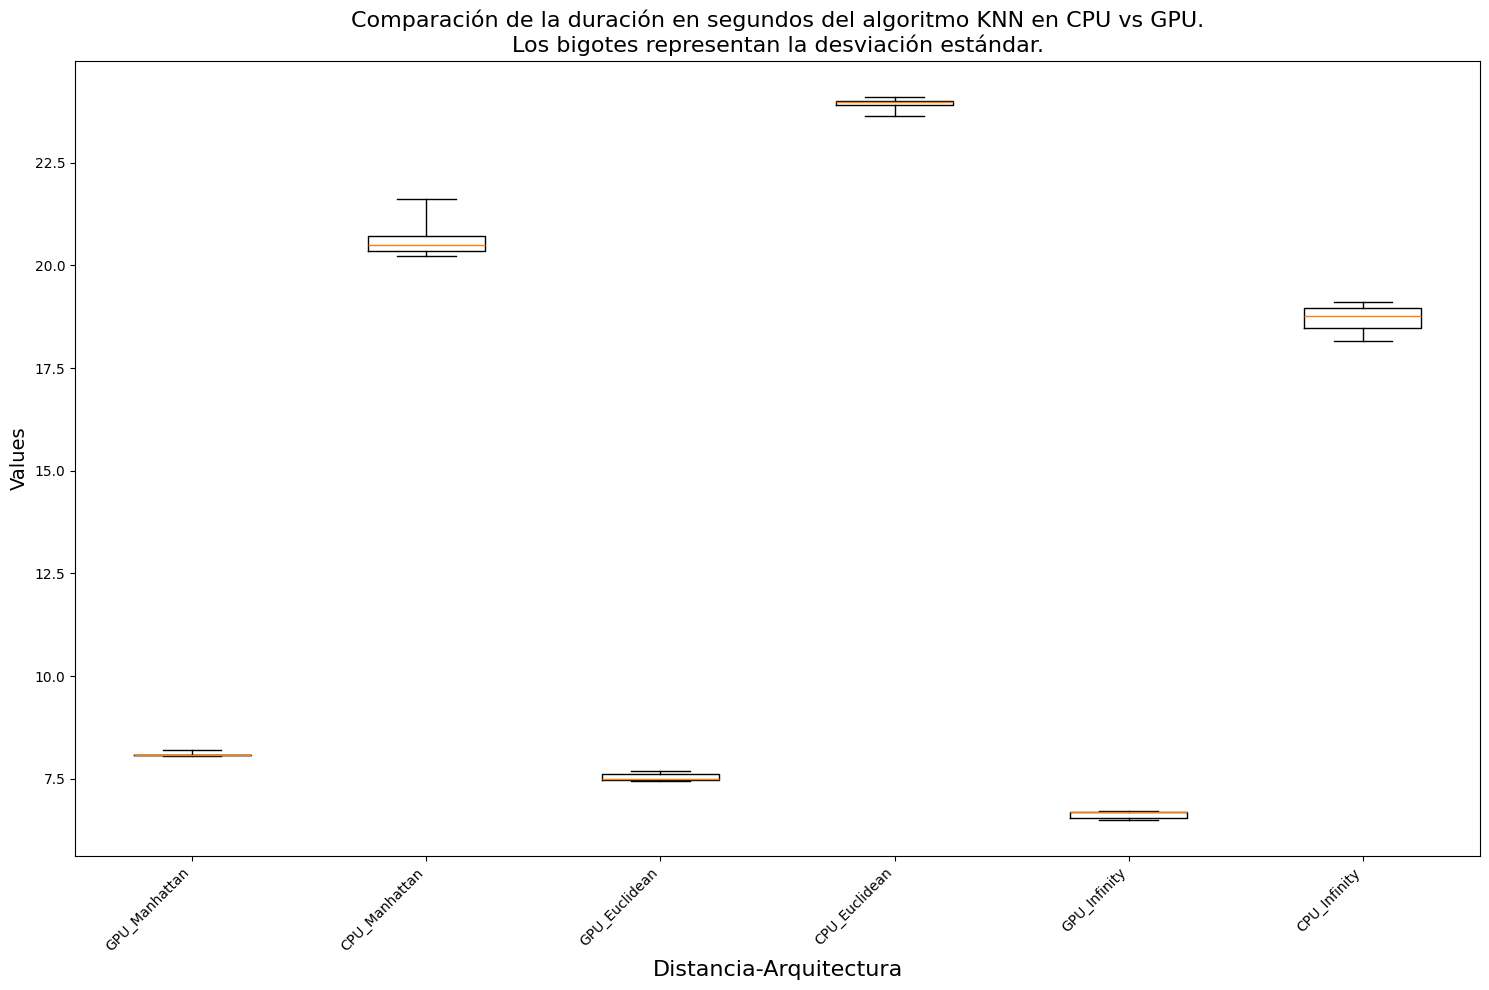
\includegraphics[width=1.1\linewidth]{img/knn_cpu_vs_gpu_segundos.png}
    \caption{Comparación de la duración en segundos del algoritmo KNN ejecutado en GPU (A100) versus CPU (L4) en Google Colab. Los bigtotes representan la desviación estándar para cada corrida.}
    \label{fig:enter-label}
\end{figure}

\item ¿Cuál distancia resulto más eficiente? 

\begin{quote}
    \textbf{R/} La distancia $\ell_{\infty}$ (infinita) parece ser más eficiente con respecto a la duración en segundos, tanto en GPU como en CPU.
\end{quote}

\item Hay algún costo en cuanto a la tasa de aciertos? Explique el porque de la diferencia en la tasa de aciertos, si la hay. 

\begin{quote}
    \textbf{R/} No se puede determinar con los resultados obtenidos que se haya sacrificado la tasa de aciertos de ninguna forma, ni por la distancia utilizada ni por el tipo de arquitectura (GPU o CPU). Para todas las configuraciones del experimento se obtuvieron resultados que parecen ser equivalentes entre sí, data sus altas tasas de aciertos superiores a $0.999$.
\end{quote}
\vspace{0.3cm}


\end{enumerate}
\end{enumerate}
\end{enumerate}

\newpage

\item Implemente el algoritmo Condensed Nearest Neighbors (CNN) para implementar de forma mas rápida el algoritmo de K-vecinos más cercano. El objetivo del algoritmo es eliminar instancias redundantes manteniendo solo los puntos críticos para preservar la estructura de decisión, y realizar inferencia mas rápido.
\begin{enumerate}
\item El algoritmo funciona como sigue, usando un conjunto de datos de entrenamiento $T$:
\begin{enumerate}
\item Comienza con un conjunto vacío condensado $C$.
\item Escoge aleatoriamente $K$ elementos y se agregan a $C$.
\item Para cada dato $\overrightarrow{x}_{i}\in T$, que al ejecutarse el algoritmo KNN usando los datos en $C$, es incorrectamente clasificado, usando como etiqueta la estimación de KNN usando $T$ (\textbf{inconsistencia
con el conjunto de datos de entrenamiento}), se agrega su vecino más cercano en $T$, hasta que la inconsistencia se arregle. De esta forma se podan los elementos que no aportan mayor información.
\end{enumerate}

\begin{tcolorbox}[breakable, size=fbox, boxrule=1pt, pad at break*=1mm,colback=cellbackground, colframe=cellborder]
\prompt{In}{incolor}{ }{\boxspacing}
\begin{Verbatim}[commandchars=\\\{\}]
\PY{k}{def}\PY{+w}{ }\PY{n+nf}{get\PYZus{}random\PYZus{}sample}\PY{p}{(}\PY{n}{data}\PY{p}{,} \PY{n}{labels}\PY{p}{,} \PY{n}{K}\PY{o}{=}\PY{l+m+mi}{7}\PY{p}{)}\PY{p}{:}
  \PY{c+c1}{\PYZsh{} data: dataset de features}
  \PY{c+c1}{\PYZsh{} labels: etiquetas de los features}
  \PY{c+c1}{\PYZsh{} k: numero de observaciones a seleccionar aleatoriamente}
  \PY{c+c1}{\PYZsh{} return: 3 tensores, uno con los features seleccionados, las etiquetas y los indices seleccionados}

  \PY{c+c1}{\PYZsh{} Genera una permutacion aleatoria de todas las observaciones}
  \PY{n}{random\PYZus{}indices} \PY{o}{=} \PY{n}{torch}\PY{o}{.}\PY{n}{randperm}\PY{p}{(}\PY{n}{data}\PY{o}{.}\PY{n}{shape}\PY{p}{[}\PY{l+m+mi}{0}\PY{p}{]}\PY{p}{)}

  \PY{c+c1}{\PYZsh{} Selecciona los primeros K índices aleatorios}
  \PY{n}{selected\PYZus{}indices} \PY{o}{=} \PY{n}{random\PYZus{}indices}\PY{p}{[}\PY{p}{:}\PY{n}{K}\PY{p}{]}

  \PY{k}{return} \PY{n}{data}\PY{p}{[}\PY{n}{selected\PYZus{}indices}\PY{p}{]}\PY{p}{,} \PY{n}{labels}\PY{p}{[}\PY{n}{selected\PYZus{}indices}\PY{p}{]}\PY{p}{,} \PY{n}{selected\PYZus{}indices}

\PY{k}{def}\PY{+w}{ }\PY{n+nf}{get\PYZus{}distancia}\PY{p}{(}\PY{n}{X}\PY{p}{,} \PY{n}{v}\PY{p}{,} \PY{n}{p}\PY{o}{=}\PY{n+nb}{float}\PY{p}{(}\PY{l+s+s1}{\PYZsq{}}\PY{l+s+s1}{inf}\PY{l+s+s1}{\PYZsq{}}\PY{p}{)}\PY{p}{)}\PY{p}{:}
  \PY{k}{if} \PY{n}{p} \PY{o}{==} \PY{n+nb}{float}\PY{p}{(}\PY{l+s+s1}{\PYZsq{}}\PY{l+s+s1}{inf}\PY{l+s+s1}{\PYZsq{}}\PY{p}{)}\PY{p}{:}
      \PY{k}{return} \PY{n}{torch}\PY{o}{.}\PY{n}{max}\PY{p}{(}\PY{n}{torch}\PY{o}{.}\PY{n}{abs}\PY{p}{(}\PY{n}{X} \PY{o}{\PYZhy{}} \PY{n}{v}\PY{p}{)}\PY{p}{,} \PY{n}{dim}\PY{o}{=}\PY{l+m+mi}{1}\PY{p}{)}\PY{o}{.}\PY{n}{values}\PY{o}{.}\PY{n}{unsqueeze}\PY{p}{(}\PY{l+m+mi}{0}\PY{p}{)}
  \PY{k}{return} \PY{n}{torch}\PY{o}{.}\PY{n}{pow}\PY{p}{(}\PY{n}{torch}\PY{o}{.}\PY{n}{sum}\PY{p}{(}\PY{n}{torch}\PY{o}{.}\PY{n}{pow}\PY{p}{(}\PY{n}{torch}\PY{o}{.}\PY{n}{abs}\PY{p}{(}\PY{n}{X} \PY{o}{\PYZhy{}} \PY{n}{v}\PY{p}{)}\PY{p}{,} \PY{n}{p}\PY{p}{)}\PY{p}{,} \PY{n}{dim}\PY{o}{=}\PY{l+m+mi}{1}\PY{p}{)}\PY{p}{,} \PY{l+m+mi}{1}\PY{o}{/}\PY{n}{p}\PY{p}{)}\PY{o}{.}\PY{n}{unsqueeze}\PY{p}{(}\PY{l+m+mi}{0}\PY{p}{)}
\end{Verbatim}
\end{tcolorbox}
\begin{tcolorbox}[breakable, size=fbox, boxrule=1pt, pad at break*=1mm,colback=cellbackground, colframe=cellborder]
\prompt{In}{incolor}{ }{\boxspacing}
\begin{Verbatim}[commandchars=\\\{\}]
\PY{k}{def}\PY{+w}{ }\PY{n+nf}{cnn\PYZus{}clasify\PYZus{}observation}\PY{p}{(}\PY{n}{C}\PY{p}{,} \PY{n}{C\PYZus{}targets}\PY{p}{,} \PY{n}{test\PYZus{}observation}\PY{p}{,} \PY{n}{p}\PY{p}{,} \PY{n}{K}\PY{p}{)}\PY{p}{:}
  \PY{c+c1}{\PYZsh{} Calcula la distancia entre la observacion de entrada y el dataset de entrenamiento}
  \PY{n}{dist} \PY{o}{=} \PY{n}{get\PYZus{}distancia}\PY{p}{(}\PY{n}{C}\PY{p}{,} \PY{n}{test\PYZus{}observation}\PY{p}{,} \PY{n}{p}\PY{p}{)}

  \PY{c+c1}{\PYZsh{} Se seleccionan los K indices con las menores distancias al conjunto condensado C}
  \PY{n}{k\PYZus{}vecinos} \PY{o}{=} \PY{n}{dist}\PY{o}{.}\PY{n}{topk}\PY{p}{(}\PY{n}{K}\PY{p}{,} \PY{n}{largest}\PY{o}{=}\PY{k+kc}{False}\PY{p}{)}

  \PY{c+c1}{\PYZsh{} Extraccion de los labels de los vecinos mas cercanos}
  \PY{n}{target\PYZus{}labels} \PY{o}{=} \PY{n}{C\PYZus{}targets}\PY{p}{[}\PY{n}{k\PYZus{}vecinos}\PY{o}{.}\PY{n}{indices}\PY{p}{[}\PY{l+m+mi}{0}\PY{p}{]}\PY{p}{]}

  \PY{c+c1}{\PYZsh{} La moda se puede usar para obtener el valor más repetido}
  \PY{c+c1}{\PYZsh{} Este valor se convierte en la etiqueta estimada}
  \PY{k}{return} \PY{n}{torch}\PY{o}{.}\PY{n}{mode}\PY{p}{(}\PY{n}{target\PYZus{}labels}\PY{p}{,} \PY{l+m+mi}{0}\PY{p}{)}\PY{o}{.}\PY{n}{values}\PY{o}{.}\PY{n}{unsqueeze}\PY{p}{(}\PY{l+m+mi}{0}\PY{p}{)}
\end{Verbatim}
\end{tcolorbox}

\begin{tcolorbox}[breakable, size=fbox, boxrule=1pt, pad at break*=1mm,colback=cellbackground, colframe=cellborder]
\prompt{In}{incolor}{ }{\boxspacing}
\begin{Verbatim}[commandchars=\\\{\}]
\PY{k}{def}\PY{+w}{ }\PY{n+nf}{evaluate\PYZus{}cnn\PYZus{}test\PYZus{}dataset}\PY{p}{(}\PY{n}{data\PYZus{}training}\PY{p}{,} \PY{n}{labels\PYZus{}training}\PY{p}{,} \PY{n}{test\PYZus{}dataset}\PY{p}{,} \PY{n}{k}\PY{o}{=}\PY{l+m+mi}{7}\PY{p}{,} \PY{n}{p}\PY{o}{=}\PY{n+nb}{float}\PY{p}{(}\PY{l+s+s1}{\PYZsq{}}\PY{l+s+s1}{inf}\PY{l+s+s1}{\PYZsq{}}\PY{p}{)}\PY{p}{)}\PY{p}{:}

  \PY{c+c1}{\PYZsh{} calcula el cnn para cada observacion del test\PYZus{}dataset}
  \PY{n}{t\PYZus{}estimated\PYZus{}dataset} \PY{o}{=} \PY{p}{[}\PY{p}{]}
  \PY{n}{C}\PY{p}{,} \PY{n}{C\PYZus{}targets}\PY{p}{,} \PY{n}{indices\PYZus{}agregados} \PY{o}{=} \PY{n}{get\PYZus{}random\PYZus{}sample}\PY{p}{(}\PY{n}{data\PYZus{}training}\PY{p}{,} \PY{n}{labels\PYZus{}training}\PY{p}{,} \PY{n}{k}\PY{p}{)}
  \PY{n}{mascara} \PY{o}{=} \PY{n}{torch}\PY{o}{.}\PY{n}{ones}\PY{p}{(}\PY{n}{data\PYZus{}training}\PY{o}{.}\PY{n}{shape}\PY{p}{[}\PY{l+m+mi}{0}\PY{p}{]}\PY{p}{,} \PY{n}{dtype}\PY{o}{=}\PY{n+nb}{bool}\PY{p}{)}
  \PY{n}{mascara}\PY{p}{[}\PY{n}{indices\PYZus{}agregados}\PY{p}{]} \PY{o}{=} \PY{k+kc}{False}  

  \PY{k}{for} \PY{n}{i}\PY{p}{,} \PY{n}{test\PYZus{}observation} \PY{o+ow}{in} \PY{n}{tqdm}\PY{p}{(}\PY{n+nb}{enumerate}\PY{p}{(}\PY{n}{test\PYZus{}dataset}\PY{p}{)}\PY{p}{)}\PY{p}{:}
    \PY{n}{t\PYZus{}consistente} \PY{o}{=} \PY{k+kc}{False}
    \PY{n}{test\PYZus{}target} \PY{o}{=} \PY{k+kc}{None}
    \PY{n}{test\PYZus{}target} \PY{o}{=} \PY{n}{cnn\PYZus{}clasify\PYZus{}observation}\PY{p}{(}\PY{n}{C}\PY{p}{,} \PY{n}{C\PYZus{}targets}\PY{p}{,} \PY{n}{test\PYZus{}observation}\PY{p}{,} \PY{n}{p}\PY{p}{,} \PY{n}{k}\PY{p}{)}
    \PY{n}{t\PYZus{}consistente} \PY{o}{=} \PY{n}{torch}\PY{o}{.}\PY{n}{equal}\PY{p}{(}\PY{n}{test\PYZus{}target}\PY{p}{,} \PY{n}{labels\PYZus{}training}\PY{p}{[}\PY{n}{i}\PY{p}{]}\PY{p}{)}

    \PY{k}{if} \PY{o+ow}{not} \PY{n}{t\PYZus{}consistente}\PY{p}{:}
      \PY{n}{training\PYZus{}filtrado} \PY{o}{=} \PY{n}{data\PYZus{}training}\PY{p}{[}\PY{n}{mascara}\PY{p}{]}
      \PY{n}{labels\PYZus{}filtrado} \PY{o}{=} \PY{n}{labels\PYZus{}training}\PY{p}{[}\PY{n}{mascara}\PY{p}{]}
      \PY{n}{dist} \PY{o}{=} \PY{n}{get\PYZus{}distancia}\PY{p}{(}\PY{n}{training\PYZus{}filtrado}\PY{p}{,} \PY{n}{test\PYZus{}observation}\PY{p}{,} \PY{n}{p}\PY{p}{)}
      \PY{n}{k\PYZus{}vecinos} \PY{o}{=} \PY{n}{dist}\PY{o}{.}\PY{n}{topk}\PY{p}{(}\PY{l+m+mi}{2}\PY{p}{,} \PY{n}{largest}\PY{o}{=}\PY{k+kc}{False}\PY{p}{)}
      
      \PY{c+c1}{\PYZsh{} Busca el siguiente vecino mas cercano que no sea la misma observacion}
      \PY{n}{nuevo\PYZus{}vecino} \PY{o}{=} \PY{n}{training\PYZus{}filtrado}\PY{p}{[}\PY{n}{k\PYZus{}vecinos}\PY{o}{.}\PY{n}{indices}\PY{o}{.}\PY{n}{squeeze}\PY{p}{(}\PY{p}{)}\PY{p}{[}\PY{o}{\PYZhy{}}\PY{l+m+mi}{1}\PY{p}{]}\PY{p}{]}\PY{o}{.}\PY{n}{unsqueeze}\PY{p}{(}\PY{l+m+mi}{0}\PY{p}{)}
      \PY{n}{etiqueta\PYZus{}nuevo\PYZus{}vecino} \PY{o}{=} \PY{n}{labels\PYZus{}filtrado}\PY{p}{[}\PY{n}{k\PYZus{}vecinos}\PY{o}{.}\PY{n}{indices}\PY{o}{.}\PY{n}{squeeze}\PY{p}{(}\PY{p}{)}\PY{p}{[}\PY{o}{\PYZhy{}}\PY{l+m+mi}{1}\PY{p}{]}\PY{p}{]}\PY{o}{.}\PY{n}{unsqueeze}\PY{p}{(}\PY{l+m+mi}{1}\PY{p}{)}

      \PY{c+c1}{\PYZsh{} Revisa que el nuevo vecino no este en C antes de agregarlo}
      \PY{k}{if} \PY{o+ow}{not} \PY{n}{torch}\PY{o}{.}\PY{n}{any}\PY{p}{(}\PY{n}{torch}\PY{o}{.}\PY{n}{all}\PY{p}{(}\PY{n}{torch}\PY{o}{.}\PY{n}{eq}\PY{p}{(}\PY{n}{C}\PY{p}{,} \PY{n}{nuevo\PYZus{}vecino}\PY{p}{)}\PY{p}{,} \PY{n}{dim}\PY{o}{=}\PY{l+m+mi}{1}\PY{p}{)}\PY{p}{)}\PY{p}{:}
        \PY{n}{C} \PY{o}{=} \PY{n}{torch}\PY{o}{.}\PY{n}{cat}\PY{p}{(}\PY{p}{(}\PY{n}{C}\PY{p}{,} \PY{n}{nuevo\PYZus{}vecino}\PY{p}{)}\PY{p}{,} \PY{n}{dim}\PY{o}{=}\PY{l+m+mi}{0}\PY{p}{)}
        \PY{n}{C\PYZus{}targets} \PY{o}{=} \PY{n}{torch}\PY{o}{.}\PY{n}{cat}\PY{p}{(}\PY{p}{(}\PY{n}{C\PYZus{}targets}\PY{p}{,} \PY{n}{etiqueta\PYZus{}nuevo\PYZus{}vecino}\PY{p}{)}\PY{p}{,} \PY{n}{dim}\PY{o}{=}\PY{l+m+mi}{0}\PY{p}{)}

      \PY{n}{mascara}\PY{p}{[}\PY{n}{k\PYZus{}vecinos}\PY{o}{.}\PY{n}{indices}\PY{o}{.}\PY{n}{squeeze}\PY{p}{(}\PY{p}{)}\PY{p}{[}\PY{o}{\PYZhy{}}\PY{l+m+mi}{1}\PY{p}{]}\PY{p}{]} \PY{o}{=} \PY{k+kc}{False}

    \PY{c+c1}{\PYZsh{} Agrega valor estimado}
    \PY{n}{t\PYZus{}estimated\PYZus{}dataset}\PY{o}{.}\PY{n}{append}\PY{p}{(}\PY{n}{test\PYZus{}target}\PY{p}{)}
  \PY{c+c1}{\PYZsh{} retorna el tensor condensado, sus etiquetas y las etiquetas estimadas}
  \PY{k}{return} \PY{n}{C}\PY{p}{,} \PY{n}{C\PYZus{}targets}\PY{p}{,} \PY{n}{torch}\PY{o}{.}\PY{n}{tensor}\PY{p}{(}\PY{n}{t\PYZus{}estimated\PYZus{}dataset}\PY{p}{)}\PY{o}{.}\PY{n}{to}\PY{p}{(}\PY{n}{data\PYZus{}training}\PY{o}{.}\PY{n}{device}\PY{p}{)}
\end{Verbatim}
\end{tcolorbox}
\item Pruebe usando los mismos datos de prueba de la función anterior, las 3 distancias usadas anteriormente. Use $K=7$. Documente el tamaño del dataset generado $S$. Hágalo para 30 corridas y compare los resultados con el algoritmo original tanto en tasa de aciertos como tiempo de ejecución en inferencia. 


\begin{table}[H]
    \centering
    \begin{tabular}{l|rrr}
    \multicolumn{4}{c}{\textbf{Tamaño conjunto $S$}}\\
    \toprule
    \textbf{Distancia}&Manhattan & Euclidean & Infinity \\    
    \midrule
    \textbf{Media}      &23089.73 & 23066.03    & 23102.30\\
    \textbf{Std. Dev.}  &61.8161  & 58.6112   & 73.6118\\
\bottomrule
\end{tabular}
    \caption{Tamaño del conjunto condensado $S$ generado por el algoritmo de CNN, para cada una de las métricas de distancias implementadas.}
    \label{tab:cnn_s_size}
\end{table}

\begin{table}[H]
    \centering
    \begin{tabular}{lrr|rr|rr}
    \toprule
    \multicolumn{7}{c}{\textbf{Tasa de Aciertos}}\\
    \midrule
    \textbf{Distancia}& \multicolumn{2}{c}{Manhattan}& \multicolumn{2}{c}{Euclidean}&\multicolumn{2}{c}{Infinity}\\
    \toprule
    &CNN&KNN& CNN&KNN & CNN&KNN\\
    \midrule
    \textbf{Media}    & 0.999671 & 0.999790 & 0.999691  & 0.999793 & 0.999700  & 0.999783 \\
    \textbf{Std. Dev} & 0.000086 & 0.000077 & 0.000069  & 0.000060 & 0.000090  & 0.000065 \\
    \bottomrule
\end{tabular}
    \caption{Comparación de las tasas de aciertos promedio con s.d. obtenidas por CNN (30 corridas) y KNN (10 corridas), ambas corridas en GPU, para cada una de las métricas de distancia.}
    \label{tab:cnn_vs_knn_tasa_aciertos}
\end{table}

\begin{table}[H]
    \centering
    \begin{tabular}{lrr|rr|rr}
    \toprule
    &\multicolumn{6}{c}{\textbf{Duración en segundos}}\\
    \midrule
    \textbf{Distancia}&\multicolumn{2}{c}{Manhattan}& \multicolumn{2}{c}{Euclidean}&\multicolumn{2}{c}{Infinity}\\
    &CNN &KNN& CNN &KNN&CNN &KNN\\
    \midrule
    \textbf{Media}&132.150336  &\textbf{8.090530} & 141.161563  &\textbf{7.543386} & 128.240465  &\textbf{6.638267} \\
    \textbf{Std. Dev.}&0.918917  &\textbf{0.040645} & 1.417119  &\textbf{0.094283} & 0.896052  &\textbf{0.091217} \\
    \bottomrule
    \end{tabular}
    \caption{Comparación de la duración en segundos promedio con s.d. obtenida tanto para CNN (30 corridas), como para KNN (10 corridas), ambas corridas en GPU, para cada una de las métricas de distancia.}
    \label{tab:cnn_vs_knn_duracion}
\end{table}

\begin{quote}
    \textbf{Comentario:} La tabla \ref{tab:cnn_s_size} evidencia como con aproximadamente un $76\%$ de los datos se puede realizar la clasificación del conjunto de datos original, lo cual cumple con la ventaja propuesta del algoritmo de clasificación Condensed Nearest Neighbors (CNN). 
    
    Al comparar las tasas de aciertos obtenidas tanto por CNN como por KNN, según muestra la tabla \ref{tab:cnn_vs_knn_tasa_aciertos}, no se puede determinar que un algoritmo sea mejor que el otro, lo cual parece indicar que el algoritmo de CNN, utilizando menos datos puede ser equivalente al KNN.

    Al analizar el tiempo de ejecución de ambos algoritmos, según la tabla \ref{tab:cnn_vs_knn_duracion}, se puede observar como nuestra implementación del CNN, fue mucho más lento que el KNN, creemos que esto es porque la implementación del CNN es menos paralelizada que el KNN, pues debemos analizar por cada observación individualmente para determinar si el conjunto $S$ es \textbf{consistente con el conjunto de entrenamiento}. 
    
    Sin embargo, una vez entrenado el algoritmo de CNN, creemos que se pueden realizar inferencias extremadamente veloces (si no se necesita actualizar $S$), y el modelo consume menos memoria que el KNN, debido a que $S \subseteq T$, donde $T$ es el conjunto de entrenamiento. En el peor de los casos, si $S \equiv T$, el consumo de memoria de CNN es igual al del KNN.
\end{quote}


\end{enumerate}
\end{enumerate}

\end{document}
